\documentclass[12pt, letterpaper]{article}
\usepackage{color}
\usepackage{natbib}
\usepackage{parskip}
\usepackage{amsmath}
\usepackage{amssymb}
\usepackage{graphicx}
\usepackage{listings}
\usepackage{setspace}
\usepackage{geometry}
\usepackage{dirtytalk}
\usepackage{subcaption}
\usepackage{indentfirst}
\usepackage{anyfontsize}
\usepackage[utf8]{inputenc}

\parindent=0.5in

\graphicspath{{./imgs/}}

\newcommand{\sorta}[1]{\lq #1\rq \,}

\definecolor{codegray}{rgb}{0.2,0.2,0.2}
\definecolor{codepurple}{rgb}{0.58,0,0.82}
\definecolor{backcolor}{rgb}{0.95,0.95,0.92}

\lstdefinestyle{scheme}
  {backgroundcolor=\color{backcolor},
  commentstyle=\color{blue},
  keywordstyle=\color{magenta},
  numberstyle=\tiny\color{codegray},
  stringstyle=\color{codepurple},
  basicstyle=\footnotesize\ttfamily,
  morekeywords={*},
  breakatwhitespace=false,
  breaklines=true,
  captionpos=t,
  keepspaces=true,
  numbers=left,
  numbersep=5pt,
  showspaces=false,
  showstringspaces=false,
  showtabs=false,
  tabsize=2,
  title=\lstname,
  language=Python
}

\lstset{style=scheme}

\doublespace{}
\title{Discussing the use of reaction diffusion equations for the simulation of physical phenomena}
\author{Simon Abrelat}
\date{\vspace{-5ex}}

\DeclareUnicodeCharacter{2212}{-}
\begin{document}

\large
{\fontsize{12}{14.4}
  {\singlespace{}
  \pagenumbering{gobble}
  \maketitle
  \begin{center}
  \vspace{4mm}
  002129--0004 \\
  \vspace{4mm}
  Extended Essay \\
  \vspace{4mm}
  May 2019 \\
  \vspace{4mm}
  Words: \\
  \end{center}
  }
}
\newpage

\pagenumbering{arabic}
\newpage
\tableofcontents
\newpage 

\section{Introduction} \label{introduction}
Reaction Diffusion equations are a type of equations with a wide range of uses and applications. They allow
for the modeling of the iterations between objects throughout space while passing through time. In other
words, they track the relationship between things over time as they spread and affect other things. This
clearly is not a technical definition but it serves to understand their purpose. It should be evident from 
the generality of their purpose that their uses are equally universal. As the name implies, they have two
\sorta{components} or sections of the equation: the reaction and the diffusion. The reaction serves as the 
relation between objects and the diffusion is the spacial component. The goal of this paper is to visually
and intuitively explain the diffusion and reaction components and to eventually tie them together to show the
complex and emergent behavior of Reaction Diffusion systems.


The thing that the Reaction Diffusion takes and manipulates or the \sorta{object} previously referred to is a
concentration variable, and the goal is to morph a concentration space. So they pass in a field of values and
returns a field or matrix of modified values. One way to think about the Reaction Diffusion is that there is
a reaction that spreads getting more \sorta{fuel} to continue the reaction. The balance between new fuel and
using up the fuel is what generates these patterns. Another examples of this sort of reaction is a
disease that starts with one person and spreads based off of who touched it and stops when everyone has
recovered or died. Given the parameters of the equation there are a variety of intuitive explanations with
different levels of accuracy or mathematical formality. 

\section{Calculus} \label{calculus}
Reaction diffusion relies on multi-variable calculus, from the partial derivative to the Laplacian 
operator that governs diffusion. Multi is a natural extension of calculus where instead of 
focusing on the accumulation or change on 1 axis, that normally being $y$, it is possible to run the calculus
operations for any
number of dimensions. This means that if a function has more than 1 input, like for 3D functions,
there is a whole new arsenal of tools and methods to analyze these equations. The limit
which fundamentally operates the same as in the 2 dimensional case. If there is a hole in the function it
would \sorta{fill in} that hole, and if there is a jump discontinuity the limit is
defined for certain directions as it approaches the discontinuity but the limit itself is undefined. Once
again, integral and derivative can be derived from the limits as in normal calculus; however, this
application will be primarily focusing on partial derivatives and other related operations. Instead
derivatives in multivariate partial derivatives are used. These are computed in a similar form to
derivatives but the inputs that are not
differentiated is treated as a constant. For use in the reaction equations the partial differential equations
behave in a similar way to differential equations except they have more inputs, but are still give the rate 
of change for a given input over a function.

\begin{singlespace}
  \begin{gather}
    \frac{\partial f}{\partial x} = \partial_x{f} = \lim_{h \to 0} \frac{f(x+h, y) − f(x,y)}{h}
    \label{eq:partX}
  \end{gather}
  \begin{gather}
    \frac{\partial f}{\partial y} = \partial_y{f} = \lim_{h \to 0} \frac{f(x, y + h) − f(x,y)}{h}
    \label{eq:partY}
  \end{gather}

  \begin{center}
   Example problem
   \begin{gather*}
    f(x, y) = xy^2 + x \\
    \partial_x f(x,y) = y^2 + 1 \\
    \partial_y f(x,y) = 2xy
   \end{gather*}
  \end{center}
\end{singlespace}

\begin{figure}[t]
  \centering
  \begin{subfigure}[b]{.6\linewidth}
    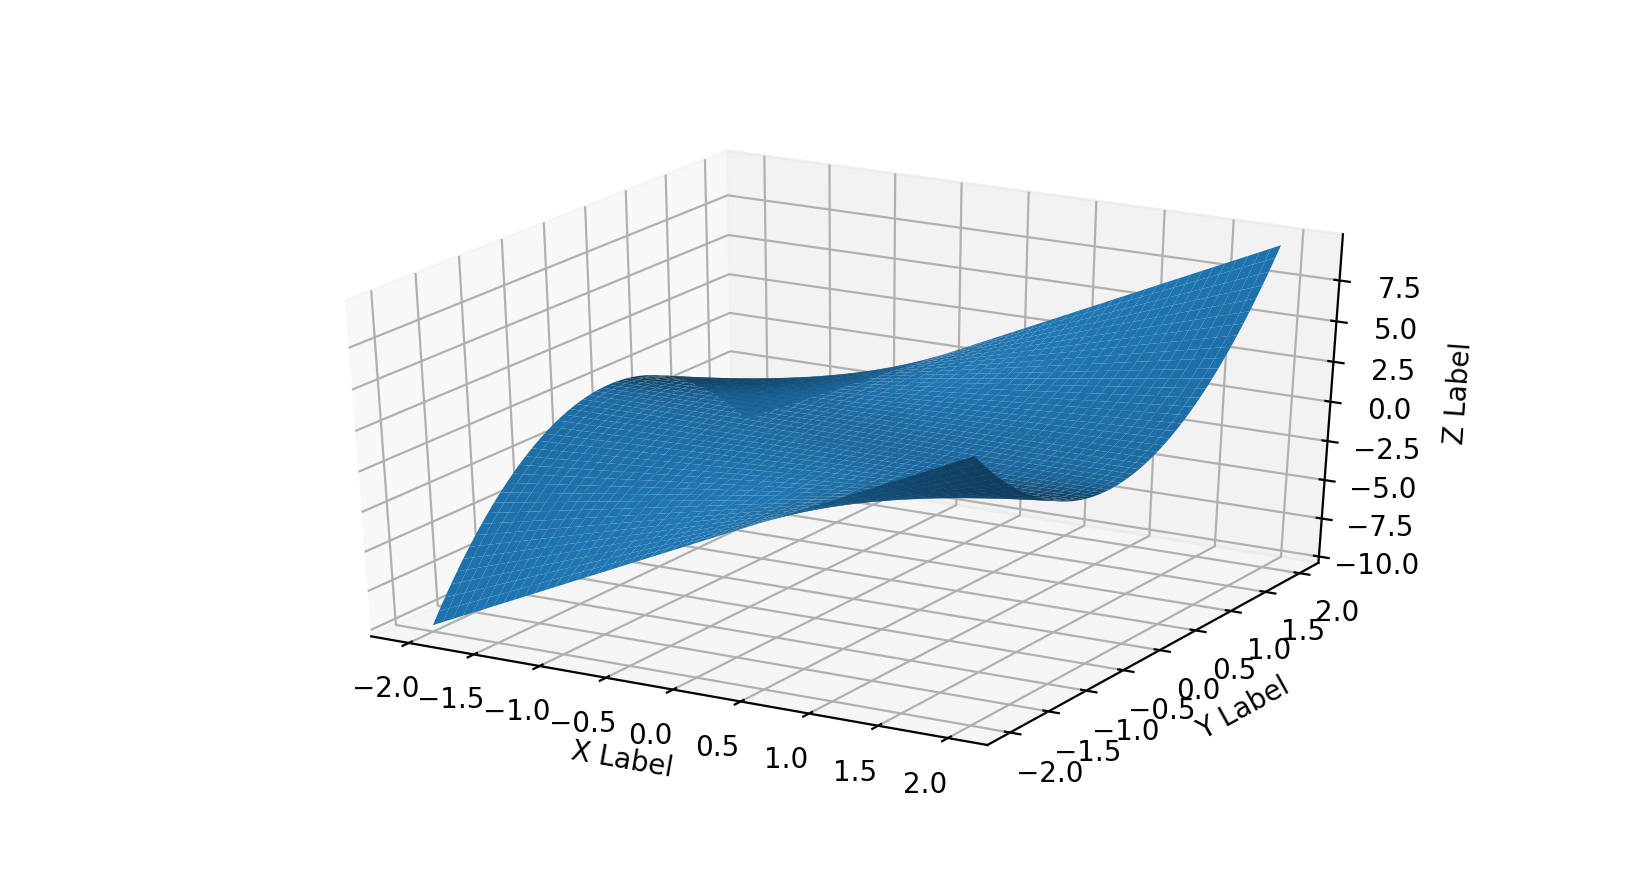
\includegraphics[width=\linewidth]{Basics/multifn}
    \caption{$f(x,y) = xy^2 + x$}
  \end{subfigure}

  \begin{subfigure}[b]{.4\linewidth}
    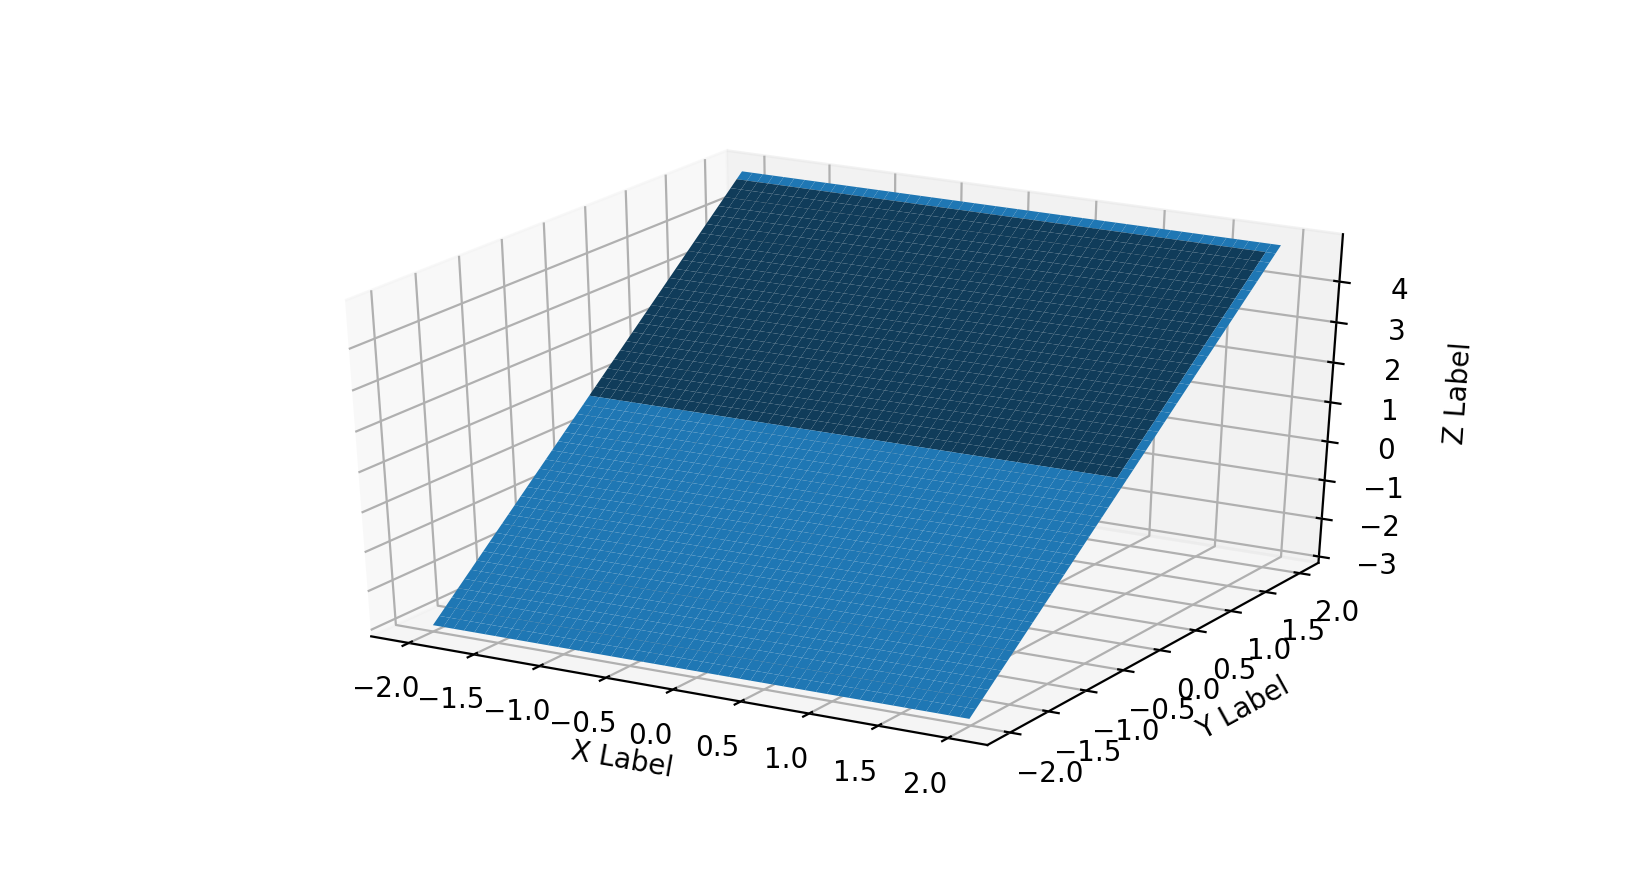
\includegraphics[width=\linewidth]{Basics/partDervX}
    \caption{$\partial_x f(x,y) = y^2 + 1$}
  \end{subfigure}
  \begin{subfigure}[b]{.4\linewidth}
    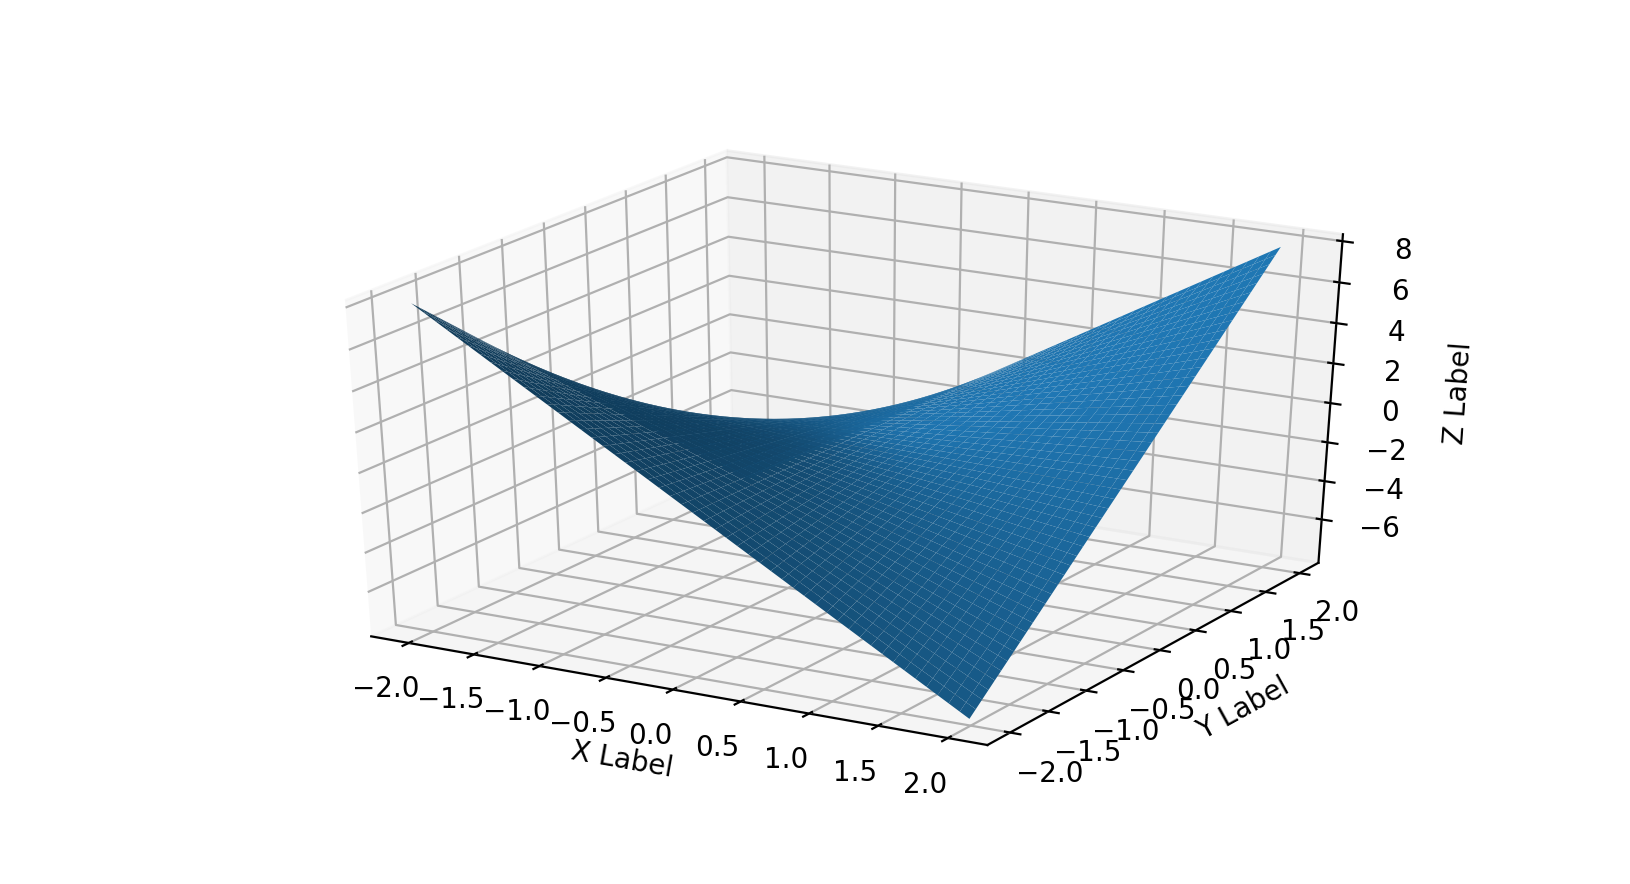
\includegraphics[width=\linewidth]{Basics/partDervY}
    \caption{$\partial_y f(x,y) = 2xy$}
  \end{subfigure}
  \caption{Example functions}
\end{figure}

Then there are directional derivatives which are similar to the partial derivatives, but instead of being in 
a component direction like along the $x$ or $y$ direction it would be in the direction of an arbitrary vector
$\vec{u}$ with components $ <a, b> $. These derivatives can be done in any number of dimensions 
(\ref{eq:NDirectional}) but for reaction diffusion formulas shown 2D cases (\ref{eq:2Directional}) matter
more.

\begin{equation}
  D_u{f(\vec{x})} = \lim_{h \to 0} \frac{f(\vec{x} + hu) − f(\vec{x})}{h}
  \label{eq:NDirectional}
\end{equation}
\begin{equation}
  D_u f = \lim_{h \to 0} \frac{f(x + ha, y+ hb) − f(x, y)}{h}
  \label{eq:2Directional}
\end{equation}
The directional derivative can also be written as a dot products.
\begin{gather*}
\begin{aligned}
  D_u f(x,y) &= a\partial_x f + b\partial_y f \\
             &= <\partial_x f, \partial_y f> * <a, b> \\
             &= <\partial_x f, \partial_y f> * u \\
             &= \nabla f(x,y) * u 
\end{aligned}
\end{gather*}

This $\nabla$, or nabla, is the sign for the grad operator. This represents a vector of all
of the partial derivatives for all of the function inputs, which is called the gradient. For example in $g(x,
y, z)$, the gradient of $g$ is the vector where each component is the partial derivative of $g$ for its
inputs $x$, $y$, and $z$. This gradient points in the direction of the \sorta{fastest increase} of the
function. So if we had a map of a mountain range the gradient of the map from a point would be the fastest
way to get to the top of the nearest mountain but not necessarily the highest mountain. The gradient is often
used for optimization problems since it can go \sorta{the highest} or local maxima in a function of any
number of variables. A common abuse of notation is to set $\nabla$ to a value (\ref{eq:nabla})

\begin{equation}
  \begin{aligned}
    \nabla &= <\frac{\partial}{\partial x}, \frac{\partial}{\partial y}, \frac{\partial}{\partial z}> \\
           &= \sum_{i=1}^{n} \vec{e}_{i} \: \frac{\partial}{\partial x_i}
  \end{aligned}
  \label{eq:nabla}
\end{equation}

\begin{figure}[!h]
  \centering
  \begin{subfigure}[b]{.45\linewidth}
    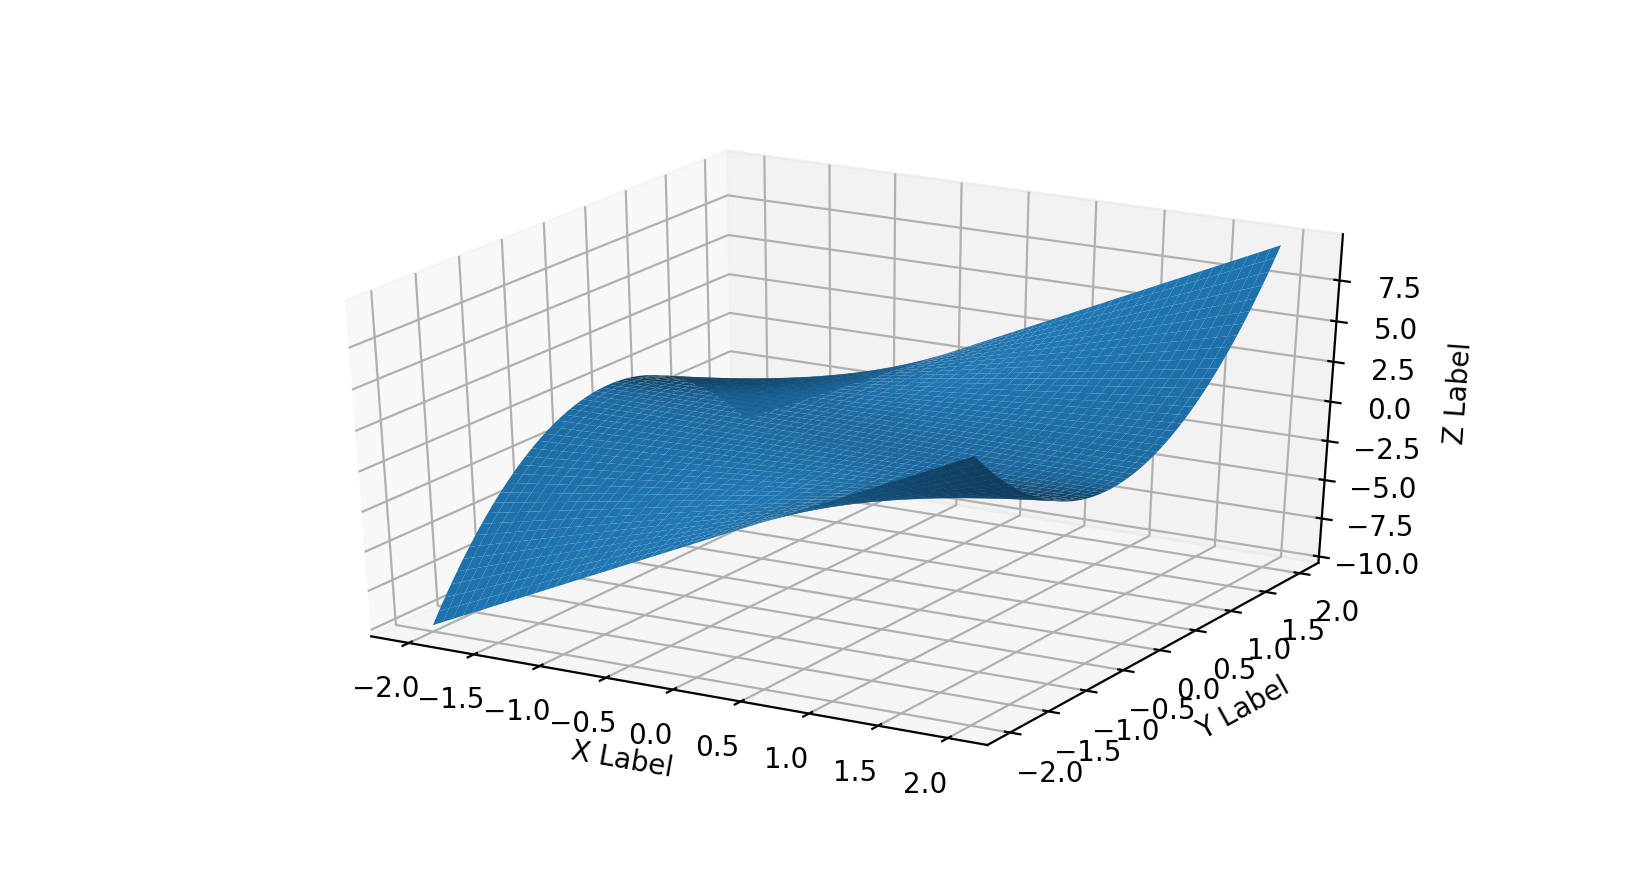
\includegraphics[width=\linewidth]{Basics/multifn}
    \caption{$f(x,y) = xy^2 + x$}
  \end{subfigure}
  \begin{subfigure}[b]{.5\linewidth}
    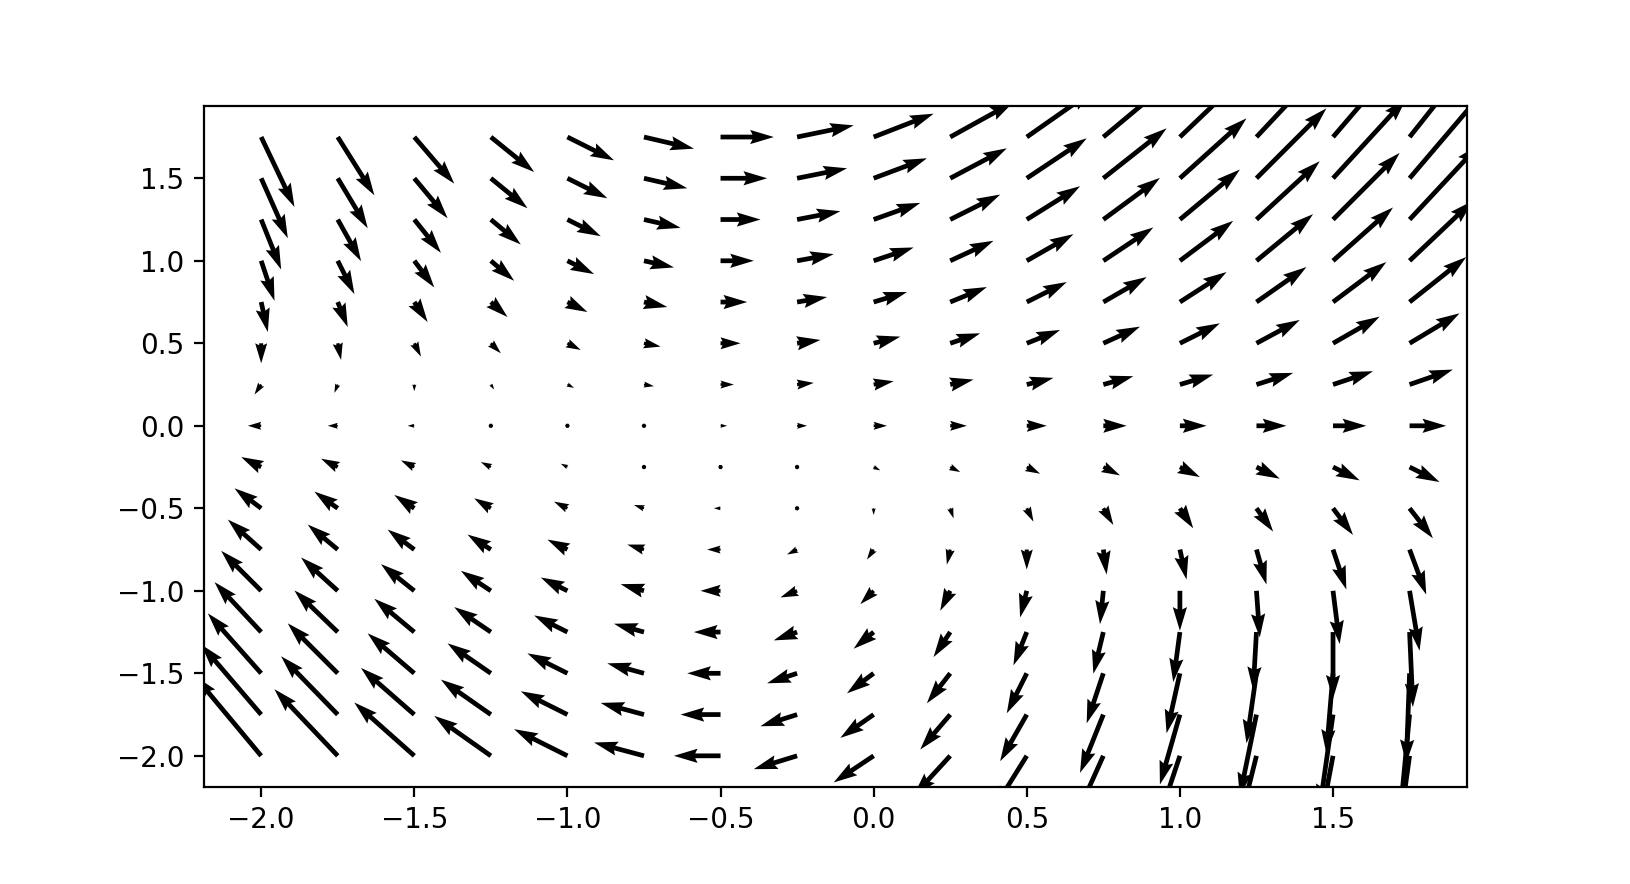
\includegraphics[width=\linewidth]{Basics/gradient}
    \caption{the gradient vector field: $\nabla * f(x,y)$}
  \end{subfigure}
\end{figure}

So the notation for the gradient makes sense because you would be treating the function f as a scalar and
multiplying it with the $\nabla$ vector. This abuse of notation since it would also make sense for the
divergence of a vector field. For a vector field the function $\mathbf{F}$ (\ref{eq:vectorFn}) would be 
a vector function where you could dot product of $\mathbf{F}$ and $\nabla$ (\ref{eq:div})

\begin{equation}
  \mathbf{F} = P\hat{\imath} + Q\hat{\jmath} + R\hat{k} \\
  \label{eq:vectorFn}
\end{equation}
\begin{equation}
  div \, \mathbf{F} = \nabla * \mathbf{F} = \frac{\partial P}{\partial x} + \frac{\partial Q}{\partial y} +
 \frac{\partial R}{\partial z}
  \label{eq:div}
\end{equation}

\begin{figure}[!h]
  \centering  
  \label{fig:div}
  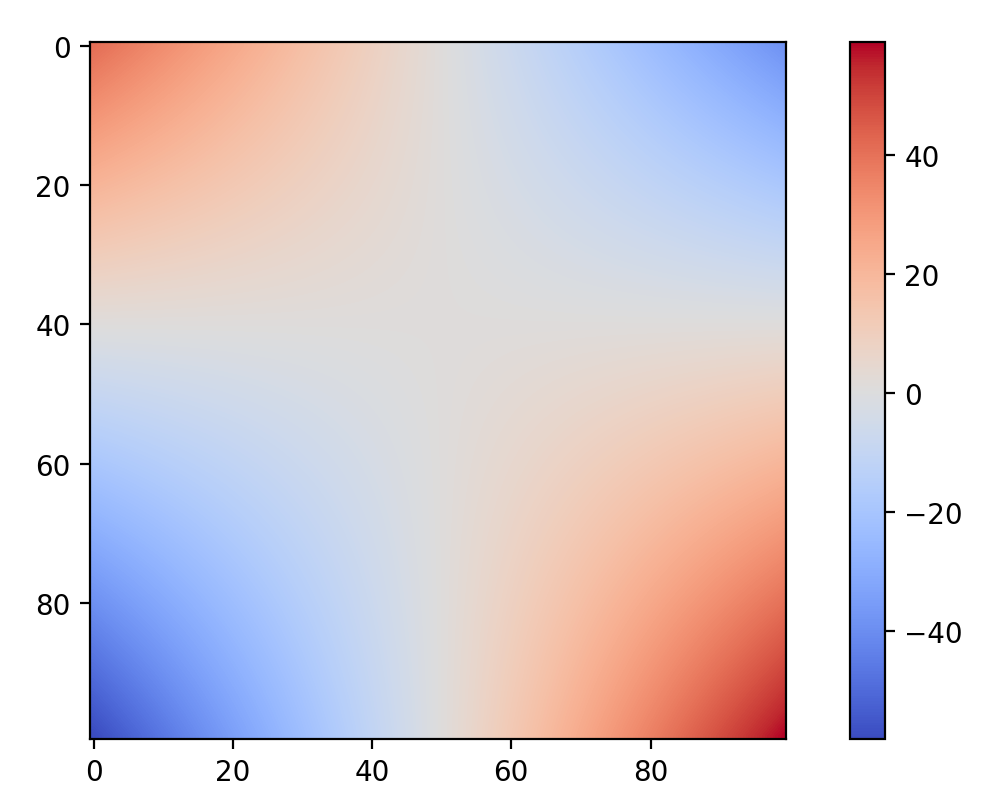
\includegraphics[width=.4\linewidth]{Basics/divergence}
  \caption{the gradient vector field: $\nabla * f(x,y)$}
\end{figure}

One can picture a vector field as being a model of fluid flow, where the vector at a point would be the
velocity of the fluid. Given this analogy, the divergence is the rate that the fluid speeds up at a
point. The divergence if positive when fluid \sorta{speeds up} and negative if it \sorta{slows down}. In a
vector field represented by all of the arrows pointing away from the origin and the arrows get larger around
a point than the divergence $>$ 0 and if the arrows are smaller or point to the origin than the divergence
$<$ 0. Both of these tools are useful but when applied together become what is needed for the diffusion part
of reaction diffusion that being the laplacian. The laplacian (\ref{eq:laplacian}) is the divergence of the
gradient of a function.
\begin{equation}
  \label{eq:laplacian}
  \begin{split}
\nabla^2 f &= \nabla * (\nabla f) \\
           &= \frac{\partial^2 f}{\partial x^2} + \frac{\partial^2 f}{\partial y^2} + \frac{\partial^2
             f}{\partial z^2} \\
           &= \sum_{i=1}^{n} \frac{\partial^2 f}{\partial x_i^2}
\end{split}
\end{equation}

This is called the Laplace operator or the Laplacian of a field because of its relation to Laplace's
Equation which has similarities to the heat transfer equation for diffusion. The reason that when put in
PDEs they exhibit this diffusion or spreading property is due to their relation to the second derivative in
normal calculus. They identify local maxima and minima but in normal calculus where the second derivative is
$0$ in both cases the laplacian is highly positive in minima and highly negative in maxima. This makes sense
because the laplacian is the sum of second partial derivatives for all of the function's inputs. In the case 
of partial derivative equations (PDEs), the laplacian \sorta{fills in} the minima and \sorta{pushes down} the
maxima. This process is what drives osmosis and heat diffusion.

\begin{equation}
  \nabla^2 \mathbf{F} = \frac{\partial^2 f}{\partial x^2} + \frac{\partial^2 f}{\partial y^2} +
  \frac{\partial^2 f}{\partial z^2} = 0
  \label{eq:laplaces}
\end{equation}

Equations that satisfies Laplace's Equation (\ref{eq:laplaces}) are called harmonic functions where at all
points the value of the laplacian equals $0$

\section{Diffusion} \label{diffusion}

Diffusion is the spread of things from high to low densities. A simple example would be heat or osmosis in 
cells. In general this is seen as spreading out. The mathematical way this is described is through a partial
differential equation using the Laplace operator, $ \nabla^2 $.

\begin{equation}
  \frac{\partial u}{\partial t} = \alpha \nabla^2 u
  \label{eq:heatDiff}
\end{equation}
\begin{equation}
  \frac{\partial u}{\partial t} = \alpha (\frac{\partial^2 u}{\partial x^2} + \frac{\partial^2 u}{\partial
  y^2} + \frac{\partial^2 u}{\partial z^2})
  \label{eq:heatDiff3}
\end{equation}

Equation~\ref{eq:heatDiff} is a simple partial differential equation that has $u(x, y, z)$ 
to determine the heat and $\alpha$ as the coefficient of thermal diffusivity. Because of the Laplace
operator, the equation does not need to show its inputs which also allows for a N-dimensional continuation.
In 3 dimensions, this equation can be expanded into equation~\ref{eq:heatDiff3}.

\begin{figure}[h]
  \caption{Heat Diffusion Progression}
  \label{fig:diffusionProgression}
  \centering
  \begin{subfigure}[b]{.21\linewidth}
    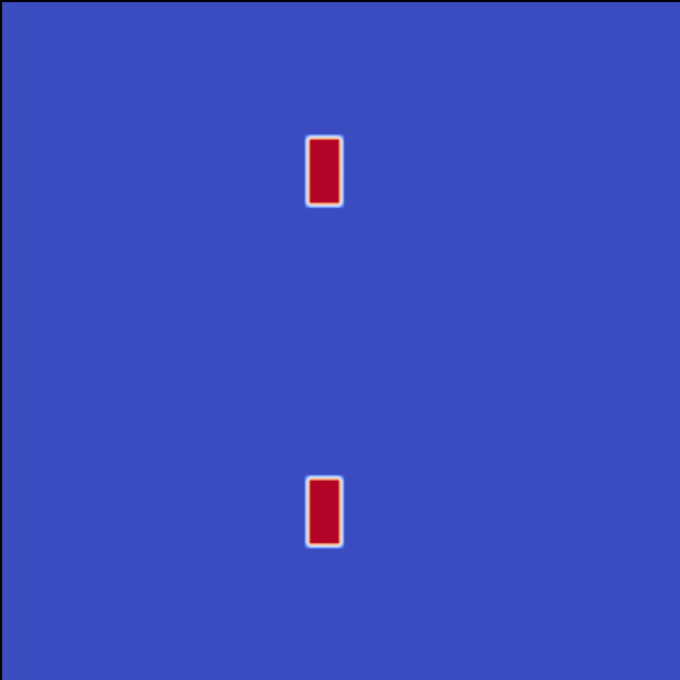
\includegraphics[width=\linewidth]{HeatProgression/diffusion0}
    \caption{$n=0$}
  \end{subfigure}
  \begin{subfigure}[b]{.21\linewidth}
    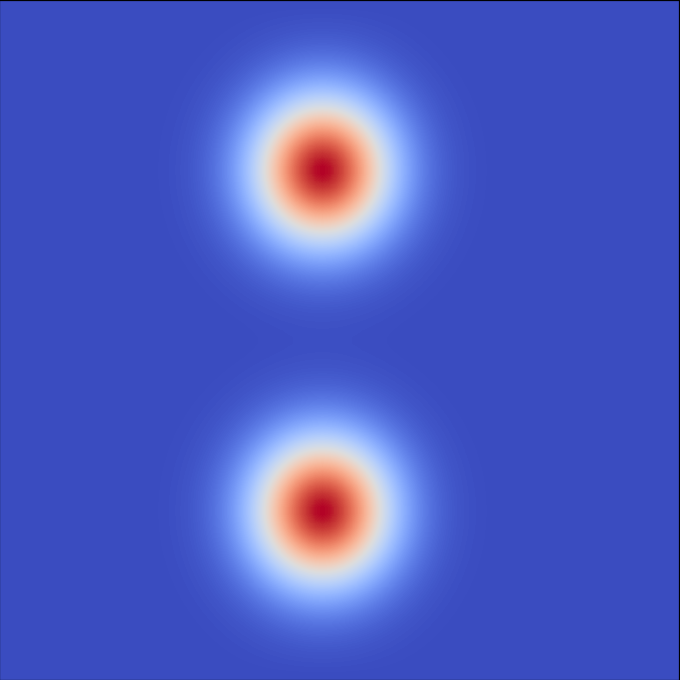
\includegraphics[width=\linewidth]{HeatProgression/diffusion1000}
    \caption{$n=1000$}
  \end{subfigure}
  \begin{subfigure}[b]{.21\linewidth}
    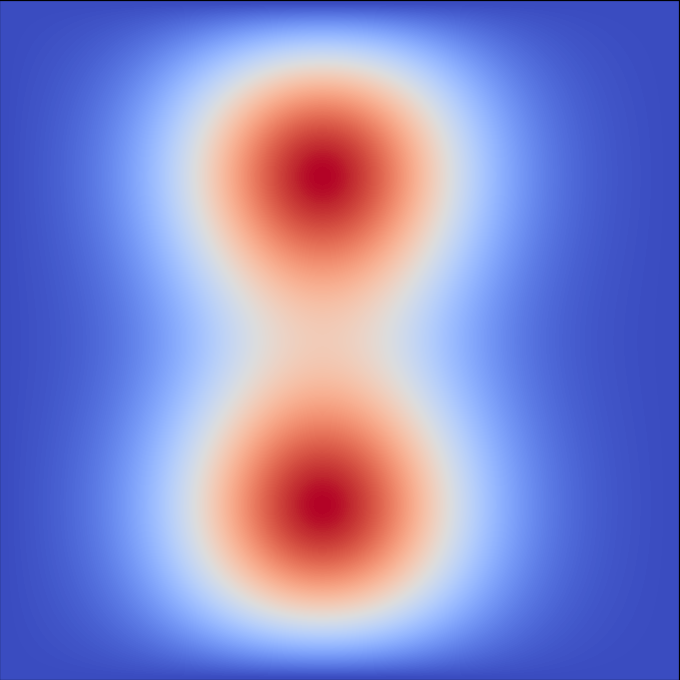
\includegraphics[width=\linewidth]{HeatProgression/diffusion5000}
    \caption{$n=5000$}
  \end{subfigure}
  \begin{subfigure}[b]{.21\linewidth}
    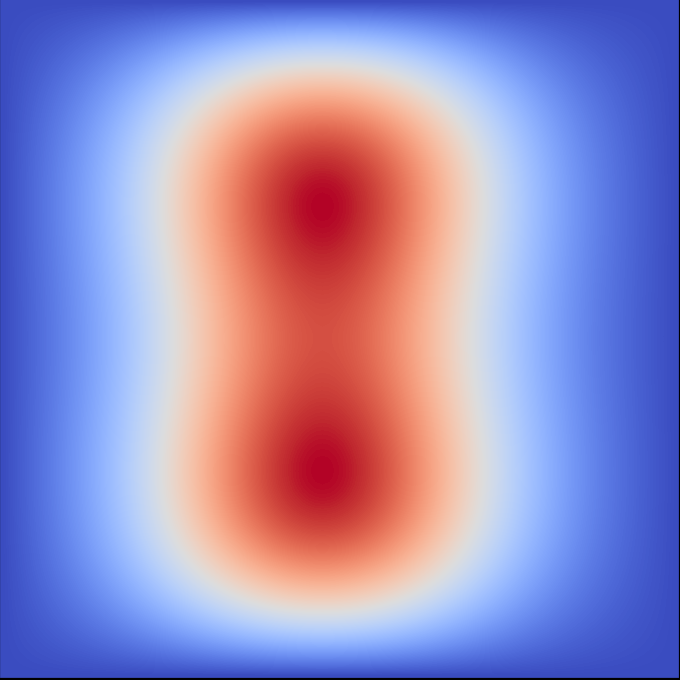
\includegraphics[width=\linewidth]{HeatProgression/diffusion8000}
    \caption{$n=8000$}
  \end{subfigure}
\end{figure}

Fig.~\ref{fig:progression} shows the progression from 2 point sources of heat that spread out, diffuse
and then eventually merge into a single blob that would continue to spread throughout the plane.

The heat diffusion equation (\ref{eq:heatDiff}) uses the laplacian which \say{pushes} the local maxima down 
and the local minima up. Later in the reaction diffusion equations, the laplacian is used to give the
equations properties based off their location and physical proximity to other elements. This diffusion
component gives reaction diffusion equations their interesting properties since previously converging
reactionary systems remain in this possibly unstable equilibrium. The reason for this is that the reactions,
spreading due to diffusion, would encounter more fuel as they go until they eventually \sorta{run out}, then
generating some homeostasis.

\section{Reaction} \label{reaction}
There things called \say{reaction systems} that typically contain multiple ordinary or partial differential 
equations. Where diffusion equations usually have only one variable, reaction systems are often 
multi-variable. There are many different examples of reaction systems, and this paper is going to focus on
the logistic equation and SIR and Lotka-Volterra models.

The most simple and generally recognized ordinary differential equation reaction system, especially relating
to population, would be the logistic equation (\ref{eq:logistic}) which is a $1$ component system that shows
the growth and maximum population of an area.

\subsection{Logistic Equation} \label{logistic}
\begin{singlespace}
  \begin{equation}\label{eq:logistic}
    \frac{dP}{dt} = rP (1 - \frac{P}{K})
  \end{equation}
  \begin{small}
$r$ is the growth rate \\
$K$ is the carrying capacity
  \end{small}
\end{singlespace}

\begin{figure}[h]
  \caption{Logistic equation $p_0=3$ $k=100$}
  \label{fig:progression}
  \centering
  \begin{subfigure}[b]{.3\linewidth}
    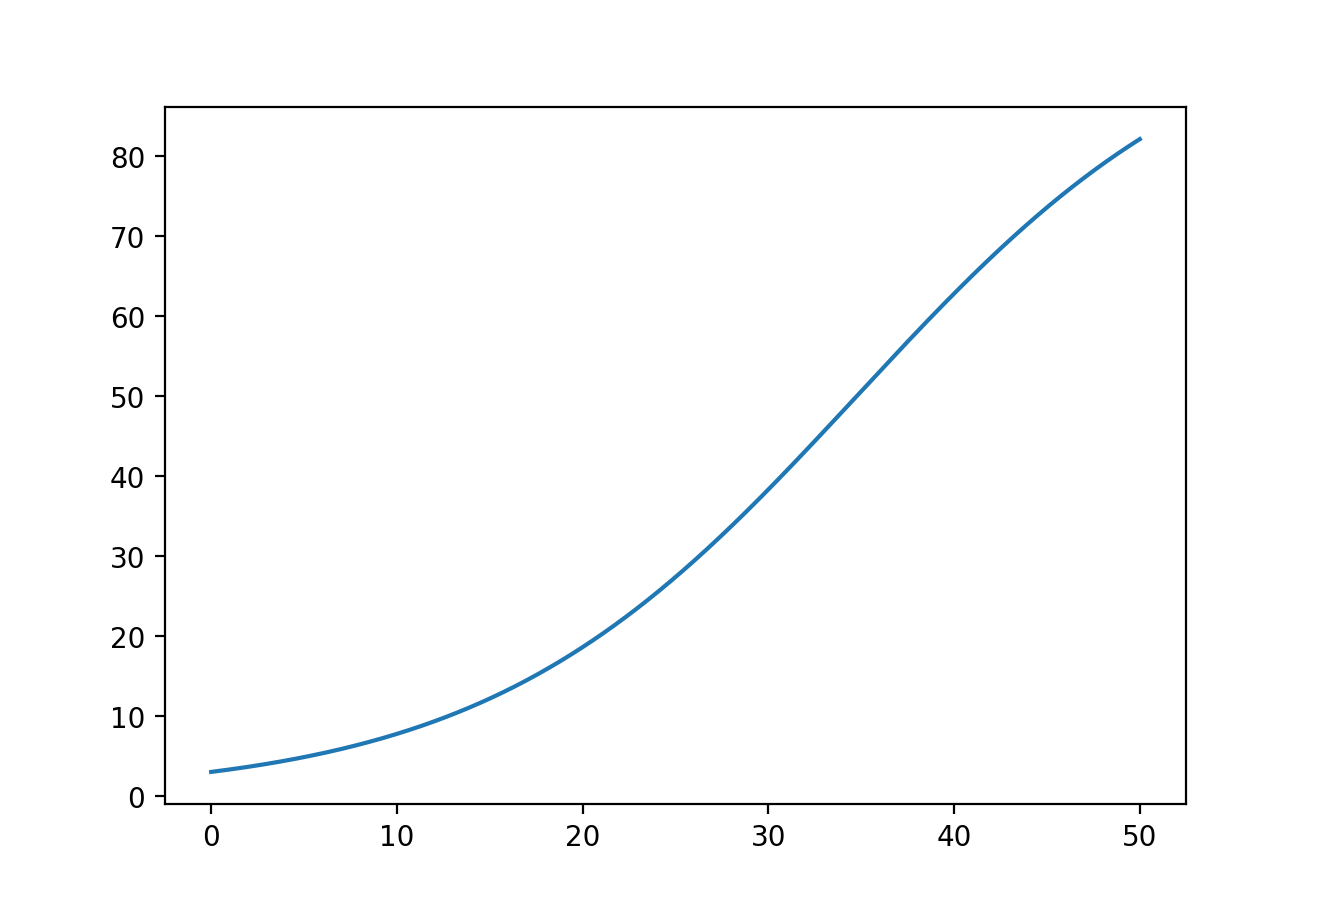
\includegraphics[width=\linewidth]{Logistic/logistic01.png}
    \caption{$r=0.1$}
  \end{subfigure}
  \begin{subfigure}[b]{.3\linewidth}
    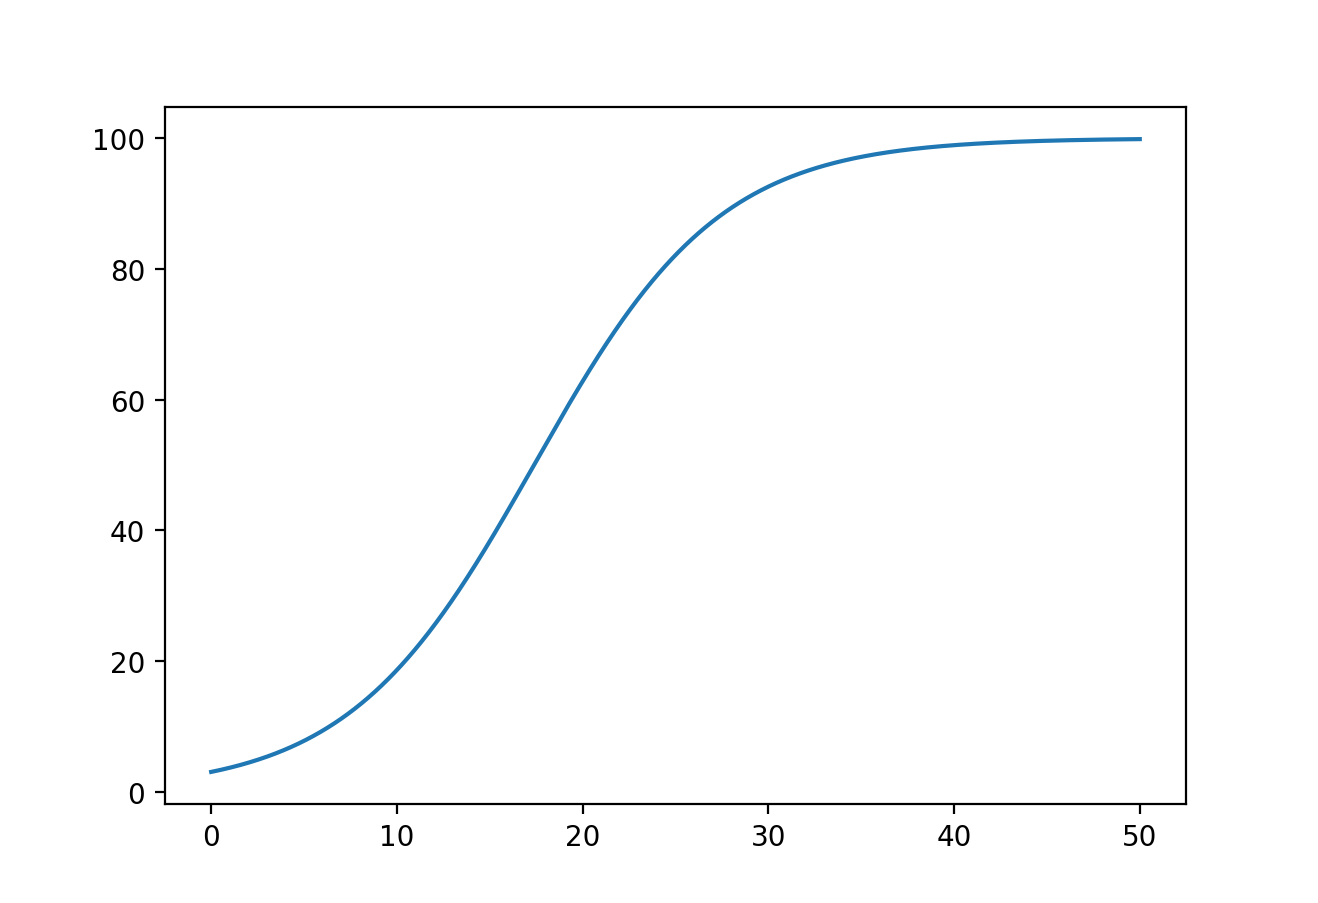
\includegraphics[width=\linewidth]{Logistic/logistic02.png}
    \caption{$r=0.2$}
  \end{subfigure}
  \begin{subfigure}[b]{.3\linewidth}
    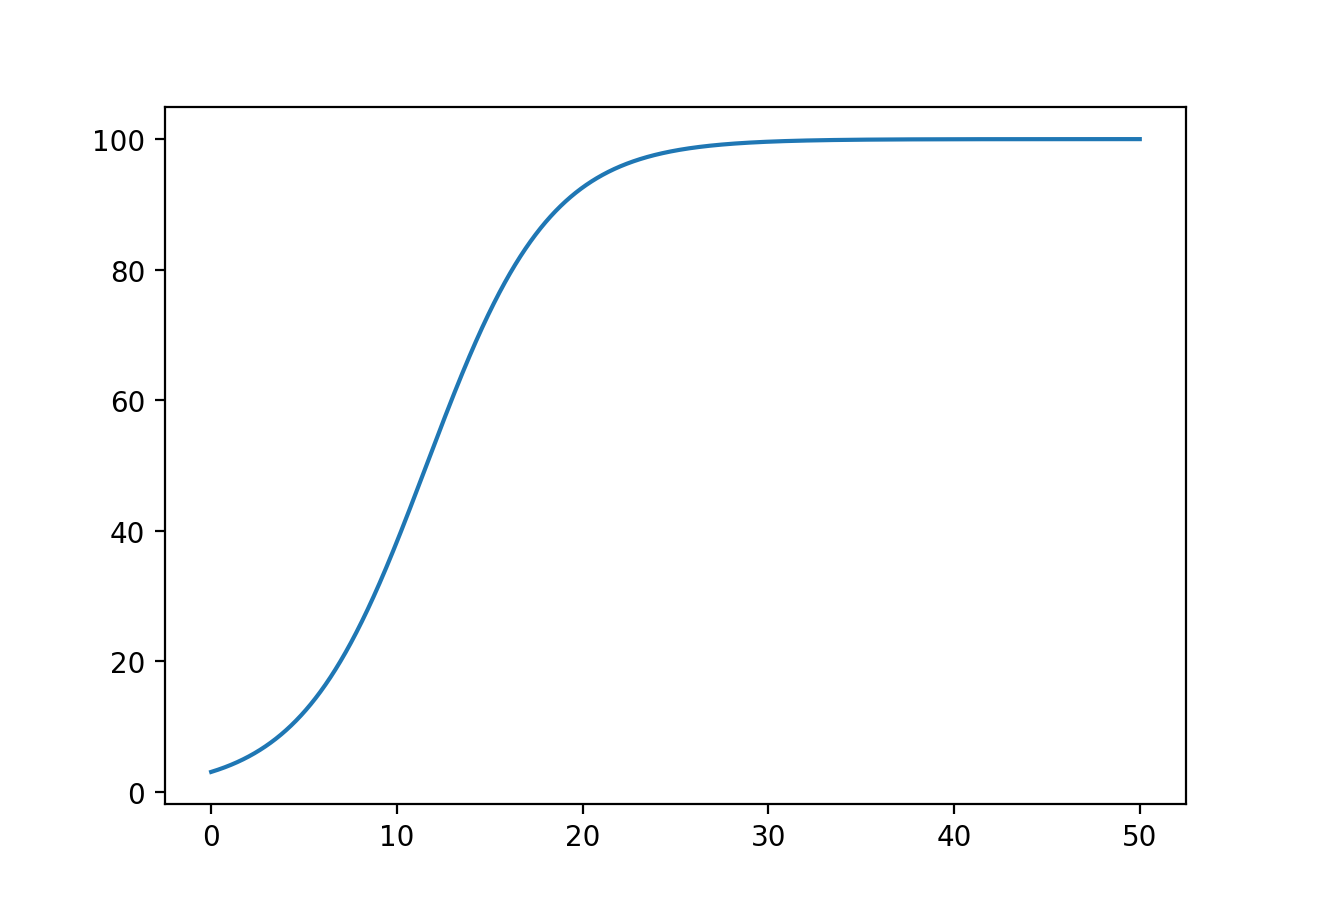
\includegraphics[width=\linewidth]{Logistic/logistic03.png}
    \caption{$r=0.3$}
  \end{subfigure}
\end{figure}

\newpage
This is the equation that describes the S-curve of growth and decay of population growth. $rP$ is the
unencumbered growth rate of the population that is clearly proportional to the current population.
$1- \frac{P}{K}$ is the limiting factor for the logistic equation. As your population approaches the carrying
capacity the growth slows, so the point they are equal and there is no more growth. If the population
increases over the carrying capacity it also pulls the population back into equilibrium This equation was
originally generated for describing Malthusian population growth, and was later rediscovered a number of
times. An examples of the use of the logistic equation is in modeling of tumor growth \citep{logisticTumor}.

\subsection{Lotka-Volterra Model} \label{lotkavolterra}
\begin{singlespace}
  \begin{equation}\label{eq:lotkaVolterra}
    \begin{split}
      &\frac{dx}{dt} = \alpha x - \beta x y \\
      &\frac{dy}{dt} = - \gamma y + \delta x y
    \end{split}
  \end{equation}
  \begin{small}
$\alpha$ is the intrinsic rate of pray population growth \\
$\beta$ is predation rate coefficient \\
$\gamma$ is the predator mortality rate. \\
$\delta$ is reproductive rate of the predators per pray eaten \\
  \end{small}
\end{singlespace}

\begin{figure}[!h]
  \caption{Examples of the Lotka-Volterra Model}
  \label{fig:lotkaVolterra}
  \begin{center}
    \begin{subfigure}[b]{.45\linewidth}
      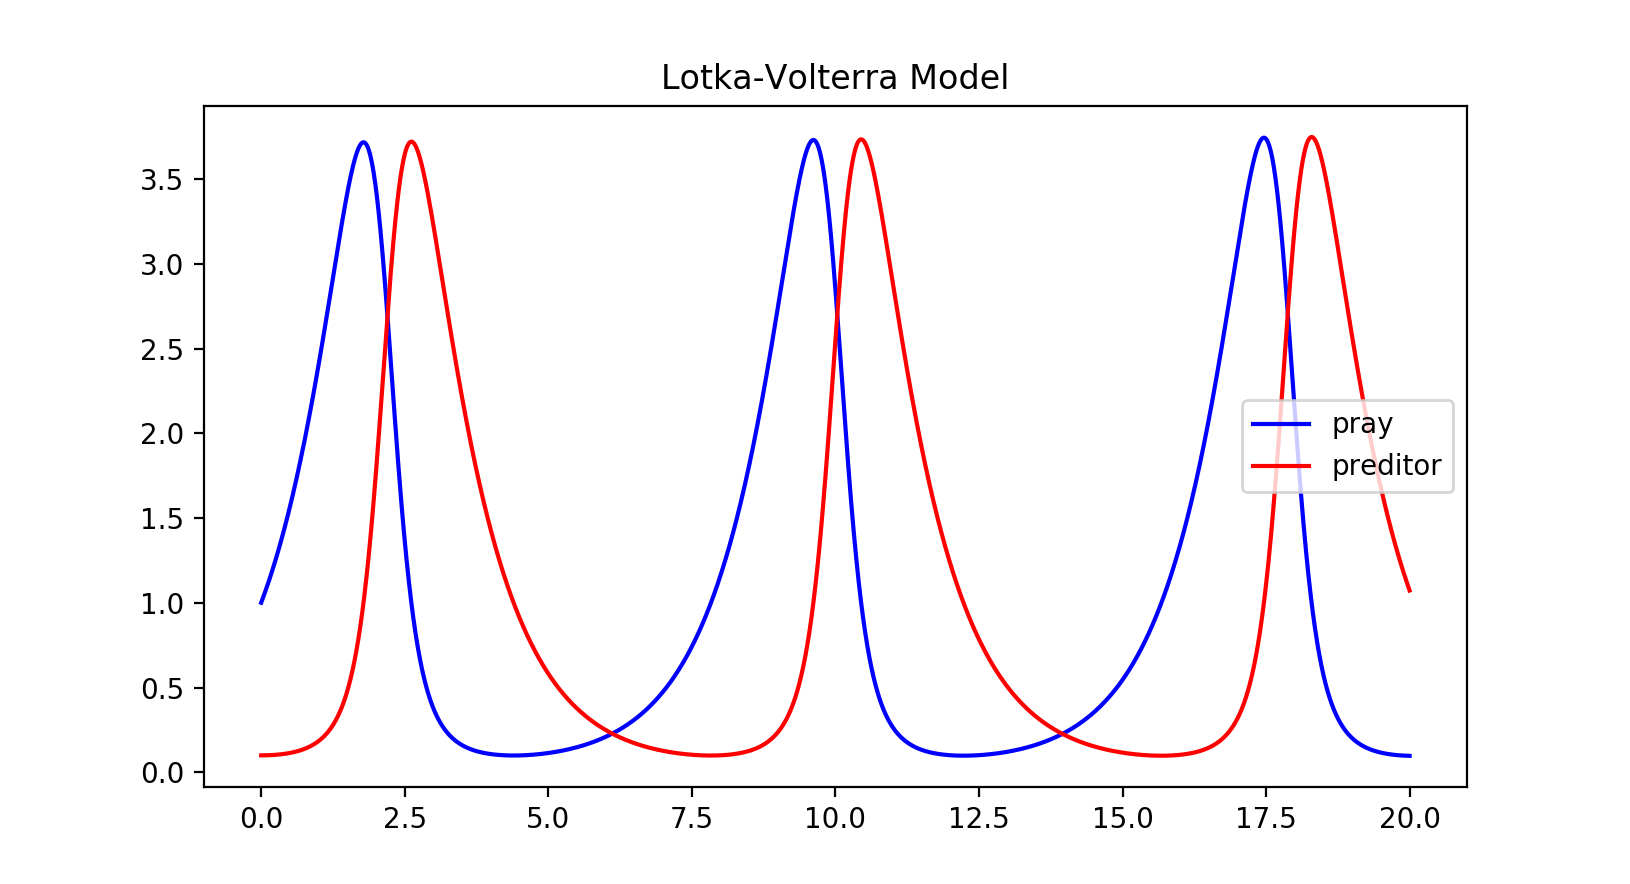
\includegraphics[width=\linewidth]{LotkaVolterra/lotkaVolterra1}
      \caption{$ \alpha = \beta = \gamma = \delta = 1$}
    \end{subfigure}
    \begin{subfigure}[b]{.45\linewidth}
      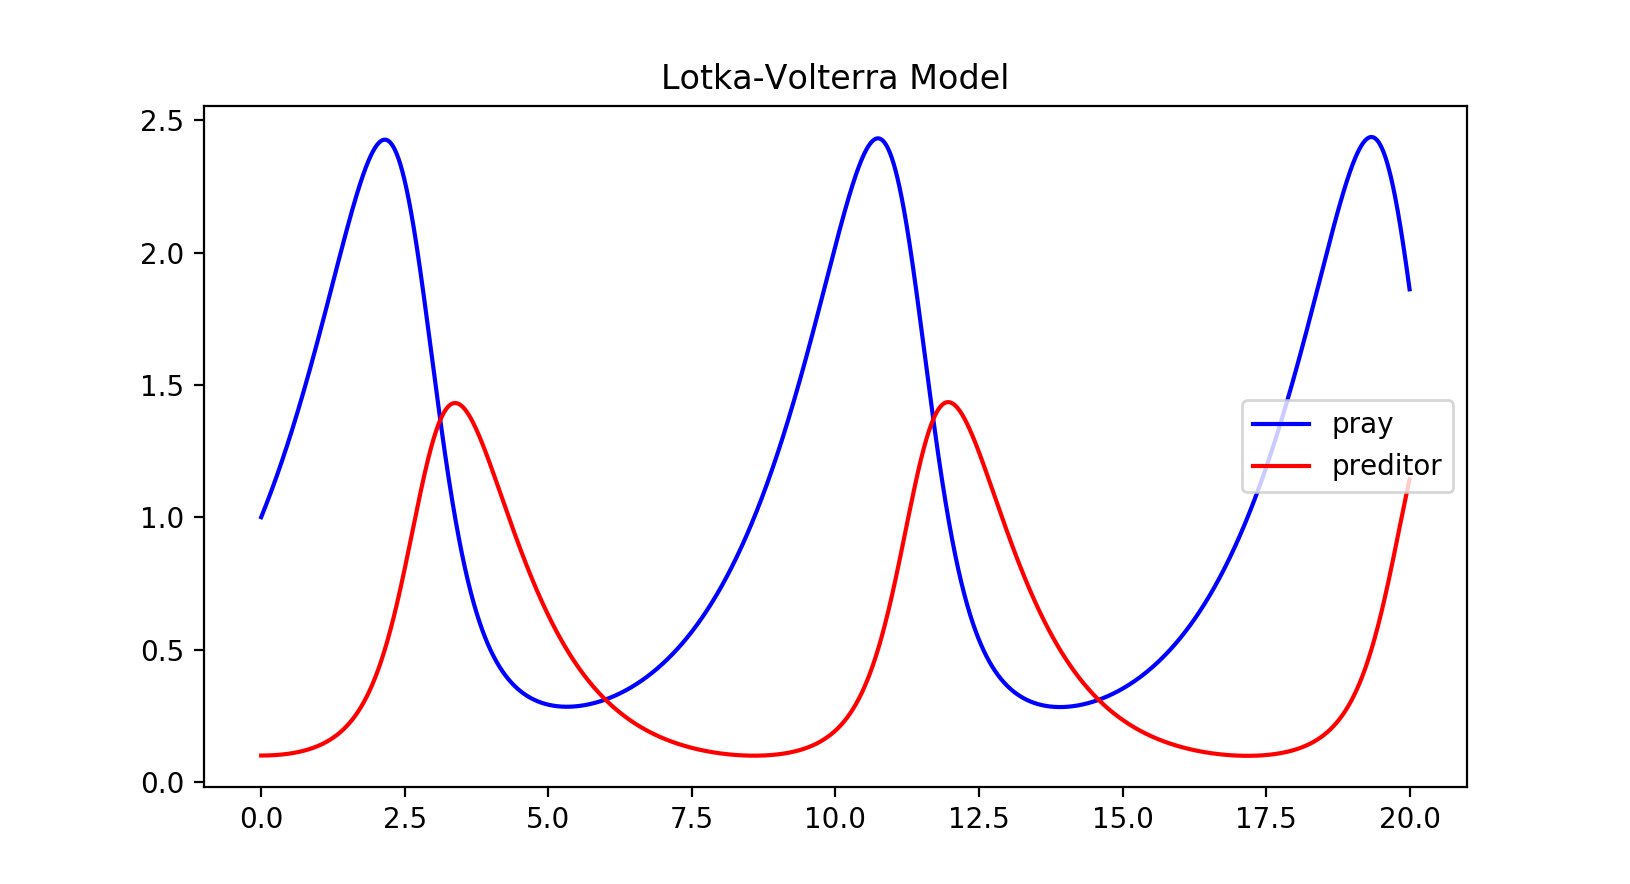
\includegraphics[width=\linewidth]{LotkaVolterra/lotkaVolterra2}
      \caption{$ \alpha = \frac{2}{3}, \beta = \frac{4}{3}, \gamma = 1, \delta = 1 $}
    \end{subfigure}
  \end{center}
\end{figure}

Another, and more complex, reaction system is the Lotka-Volterra model (\ref{eq:lotkaVolterra}). This is used
to model the populations of predators and pray as they grow and shrink in a cyclical manner, making it a 2
component system, in the case $x$ for prey and $y$ for predators. This is one of the earliest Predator-Pray
models based on sound mathematical principles. There are some problems with such a simple model, but the
biggest issue is in reality populations reach an equilibrium but this model is cyclic; however, there are
also cases were there is a cyclic growth off to infinity becoming unstable \citep{lotkaVolterra}. These
issues mainly come from a lack of 
gender differences, size effects like overpopulation and resources, and a variety of outside influences. That
is why this is only used to describe specific predator-prey examples like hare and lynx populations. The
benefit of such a simple model is the simple explanation. For prey, $\alpha x$ is clearly the unencumbered
growth rate and $-\beta x y$ is the rate of predation that is influenced by the size of both the predator and
prey populations. The predators explanation is a little more complicated. For predators, the $\delta x y$ is
the increase in predator population given that each predator reproduces at a rate $\delta$ per prey eaten; 
such that, each predator eats all the prey and produces proportional to that. The $- \gamma y$ is simply the
mortality rate for the predators.

\subsection{SIR Model} \label{sir}
\begin{singlespace}
  \begin{equation}\label{eq:SIR}
    \begin{split}
      &\frac{dS}{dt} = -\beta s i \\
      &\frac{dI}{dt} = \beta s i - \kappa r \\
      &\frac{dR}{dt} = \kappa r
    \end{split}
  \end{equation}
  \begin{small}
$\kappa$ is the number of days until recovery \\
$\beta$ is the number of days needed to be in contact to spread
  \end{small}
\end{singlespace}

\begin{figure}[!h]
  \caption{Examples of SIR model}
  \label{fig:SIR}
  \begin{center}
    \begin{subfigure}[b]{.35\linewidth}
      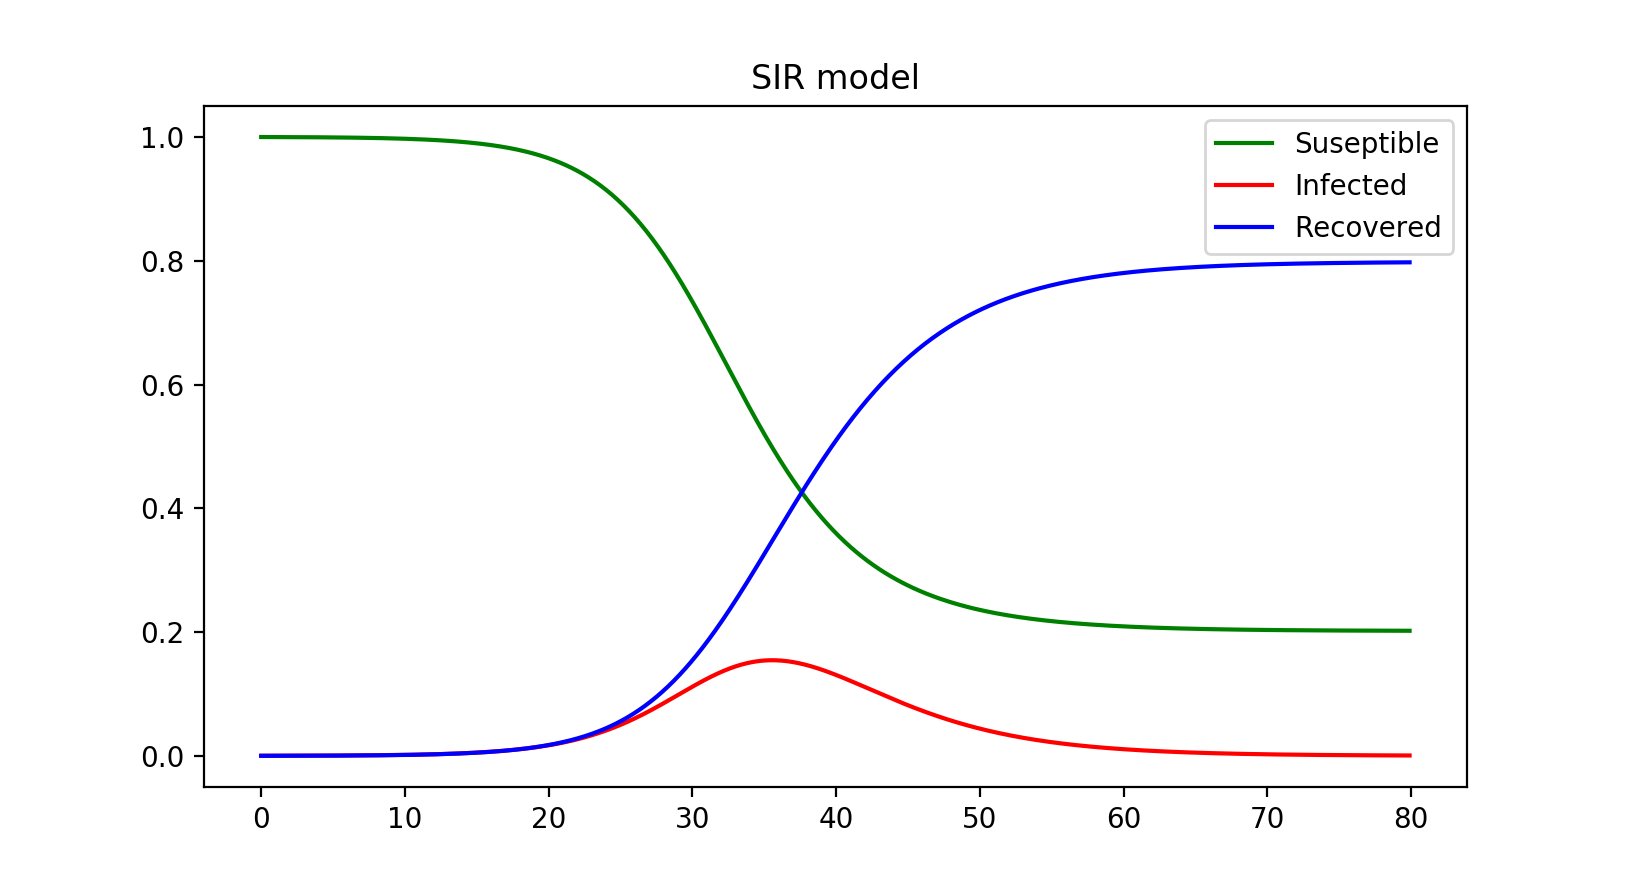
\includegraphics[width=\linewidth]{SIR/SIR_Start}
      \caption{$\kappa = \frac{1}{3}, \beta = \frac{1}{2}$}
    \end{subfigure}
    \begin{subfigure}[b]{.35\linewidth}
      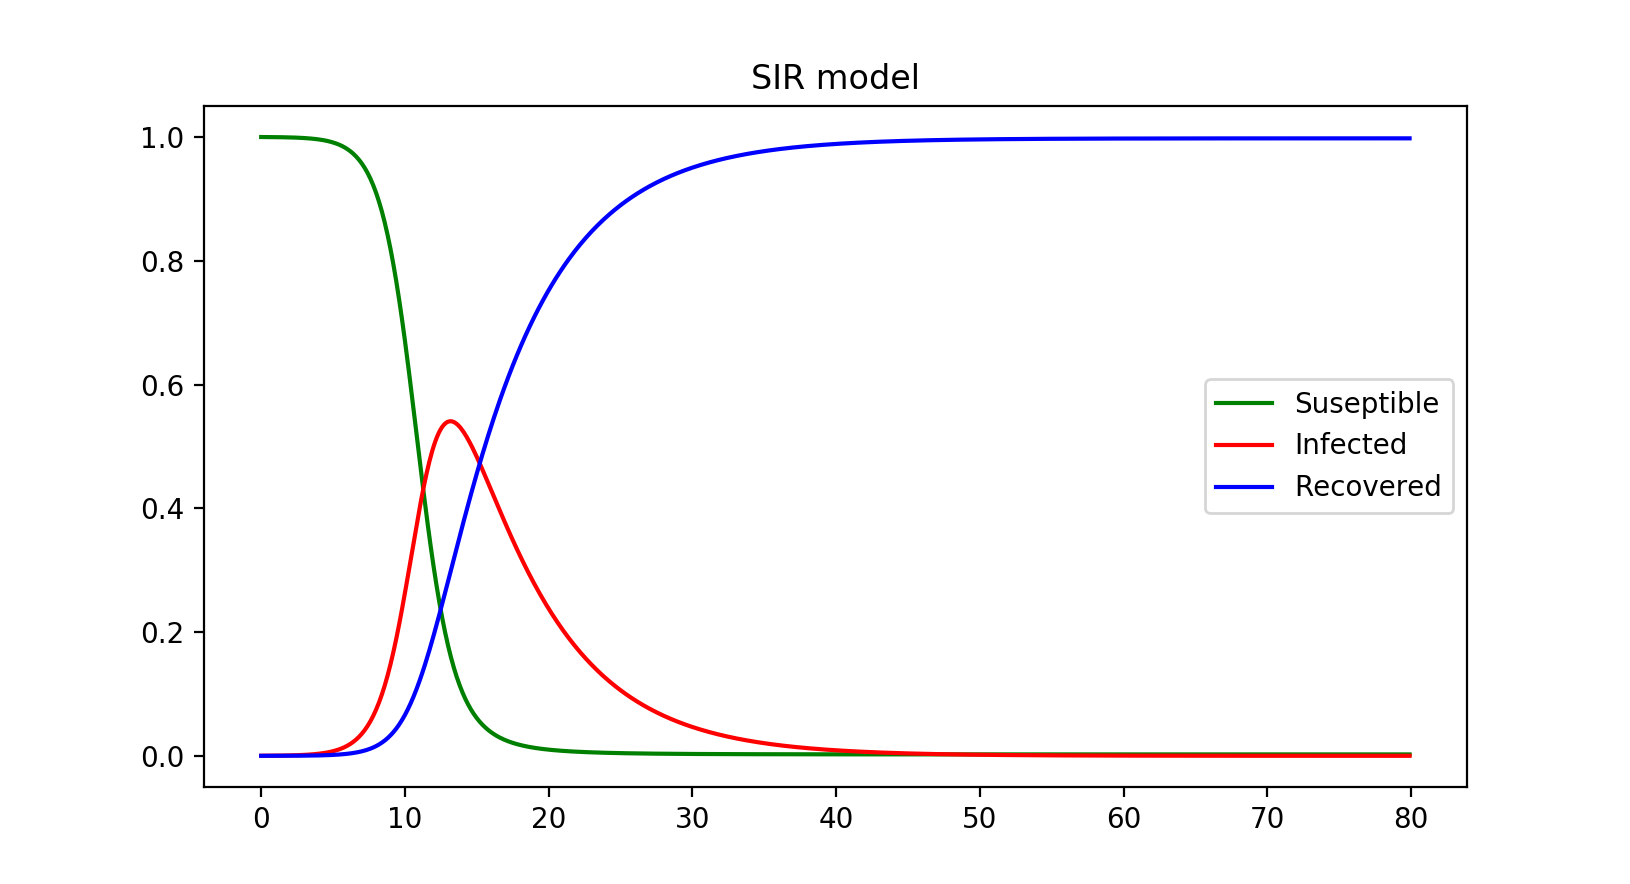
\includegraphics[width=\linewidth]{SIR/SIR_Epi}
      \caption{$\kappa = \frac{1}{6}, \beta =  1$}
    \end{subfigure}
  \end{center}
\end{figure}

The SIR model (\ref{eq:SIR}), or Susceptible-Infected-Recovered Model, is a computational epidemiology and
serves as the core of other more advanced models, despite already having 3 components. This model is
fairly intuitive. The susceptible equation is similar to the predation in the Lotka-Volterra Model, were the
population decreases by the rate of spread times the infected and the susceptible $- \beta s i$. That means
that if the size of the infected or susceptible populations are low, then there are few new cases of 
illness. The recovering is simply decreasing by the recovery rate times infected $\kappa r$.  Then, the
infected change is equal to the number gained of new infected minus the number lost who recovered $\beta s
i - \kappa r$. In figure~\ref{fig:SIR}a it shows a normal illness if no strong where in a small population
similar to a school there is a wave that infect most people but is not an epidemic. Then, 
figure~\ref{fig:SIR}b is an example of an epidemic.

\section{Reaction Diffusion} \label{reactiondiffusion}

\begin{singlespace}
  \begin{equation}
    \label{eq:genRD}
    \frac{\partial \vec{q}}{\partial t} = − \underline{\underline{\mathbf{D}}} \nabla^2 \vec{q} + R(\vec{q})
  \end{equation}
  \begin{small}
    $\underline{\underline{\mathbf{D}}}$ is a diagonalized weight matrix \\
    $\vec{q}$ is a vector of inputs given a time \\
    $R(\vec{q})$ is a function that takes into account local reactions
  \end{small}
\end{singlespace}

Reaction Diffusion is then the merger of diffusion and reaction systems, with emergent properties. The
generalized formula (\ref{eq:genRD}) works in any number of dimensions and with any number of components. To
limit algorithmic complexity, the 1 and 2 dimensional cases will be focused on. The $R(\vec{q})$ is a vector
equation that represents the reaction systems described in section~\ref{reaction}. To complete the name, the 
$\underline{\underline{\mathbf{D}}} \nabla^2 \vec{q}$ then represents the diffusion for any number of
dimensions, exactly like heat diffusion described in section~\ref{diffusion}.

\subsection{Fisher's equation} \label{fisher}
The first reaction diffusion system is Fisher's equation (\ref{eq:fisher}) which is a 1 component, 1
dimensional system that represents the wave front switching between equilibrium states, such as a switch of
dominate traits \citep{fisher}.

\begin{equation}
  \label{eq:fisher}
  \frac{\partial u}{\partial t} - D \frac{\partial^2 u}{\partial x^2} = ur(1 - u) 
\end{equation}

\begin{figure}[h]
  \caption{Fisher Equation Example}
  \label{fig:fisherGraphs}
  \centering
  \begin{subfigure}[b]{.23\linewidth}
    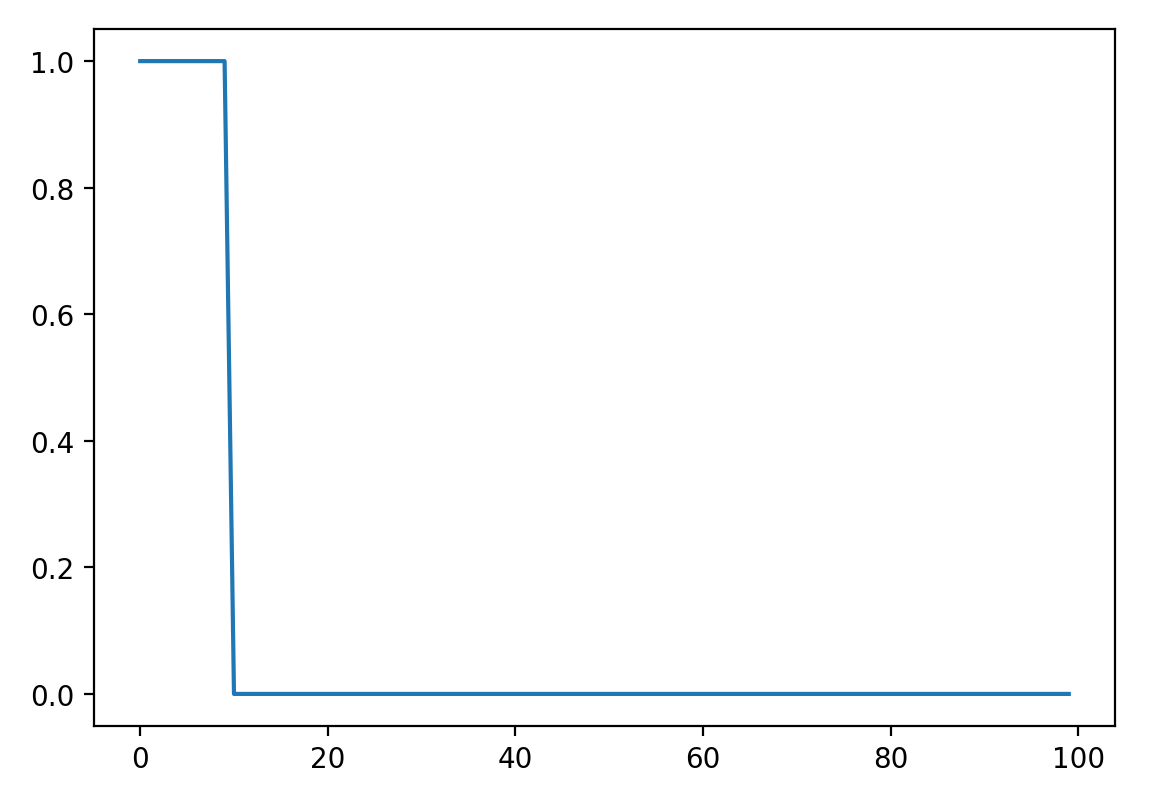
\includegraphics[width=\linewidth]{Fisher/f0.png}
    \caption{$t=0$}
  \end{subfigure}
  \begin{subfigure}[b]{.23\linewidth}
    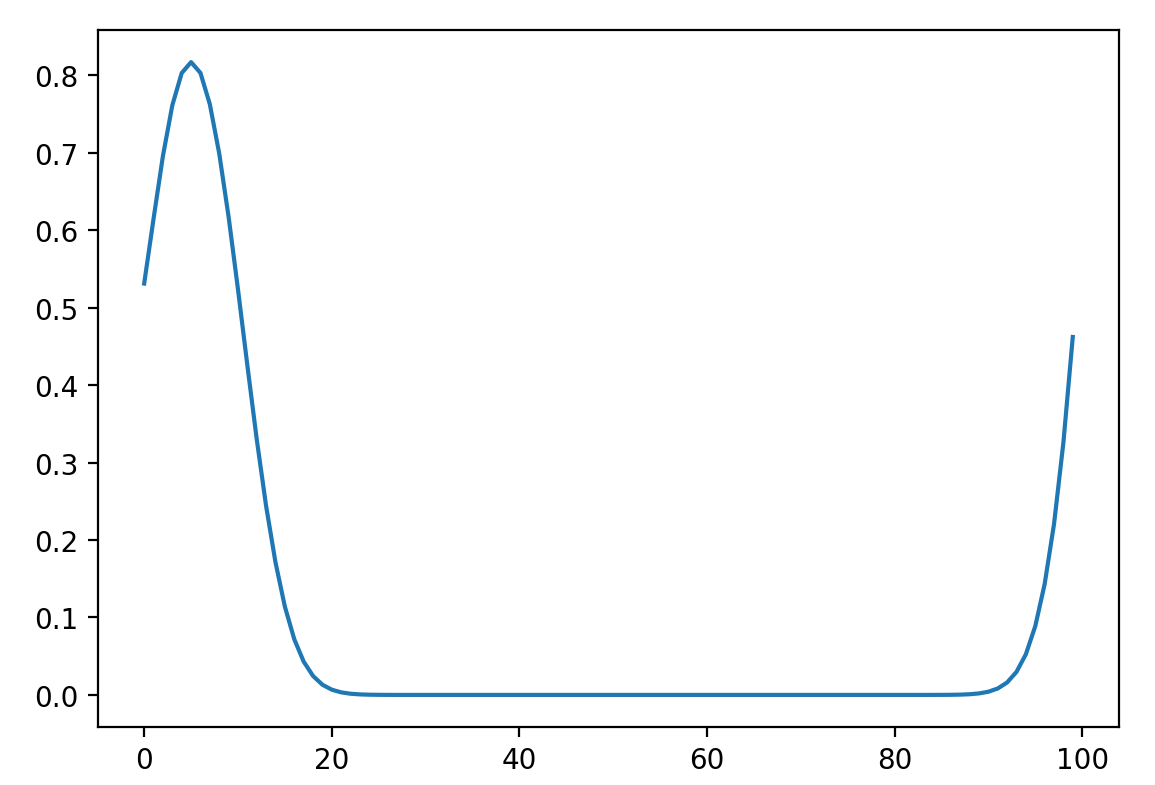
\includegraphics[width=\linewidth]{Fisher/f50.png}
    \caption{$t=50$}
  \end{subfigure}
  \begin{subfigure}[b]{.23\linewidth}
    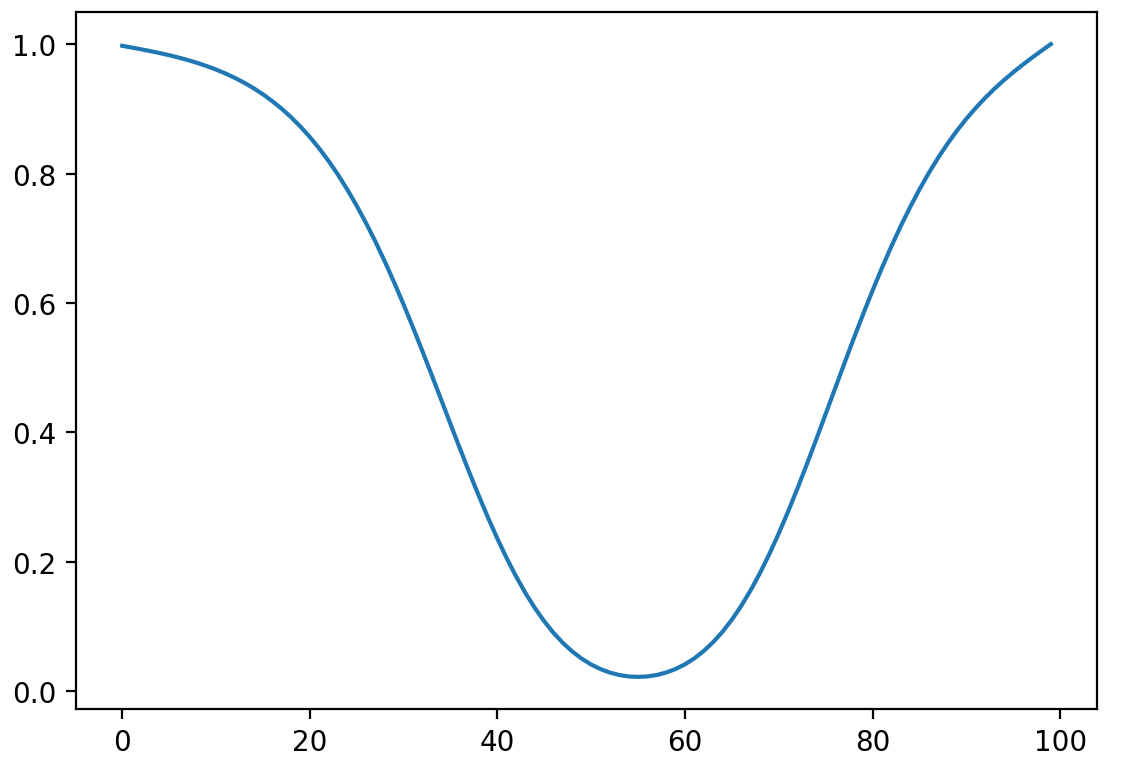
\includegraphics[width=\linewidth]{Fisher/f500.png}
    \caption{$t=500$}
  \end{subfigure}
  \begin{subfigure}[b]{.23\linewidth}
    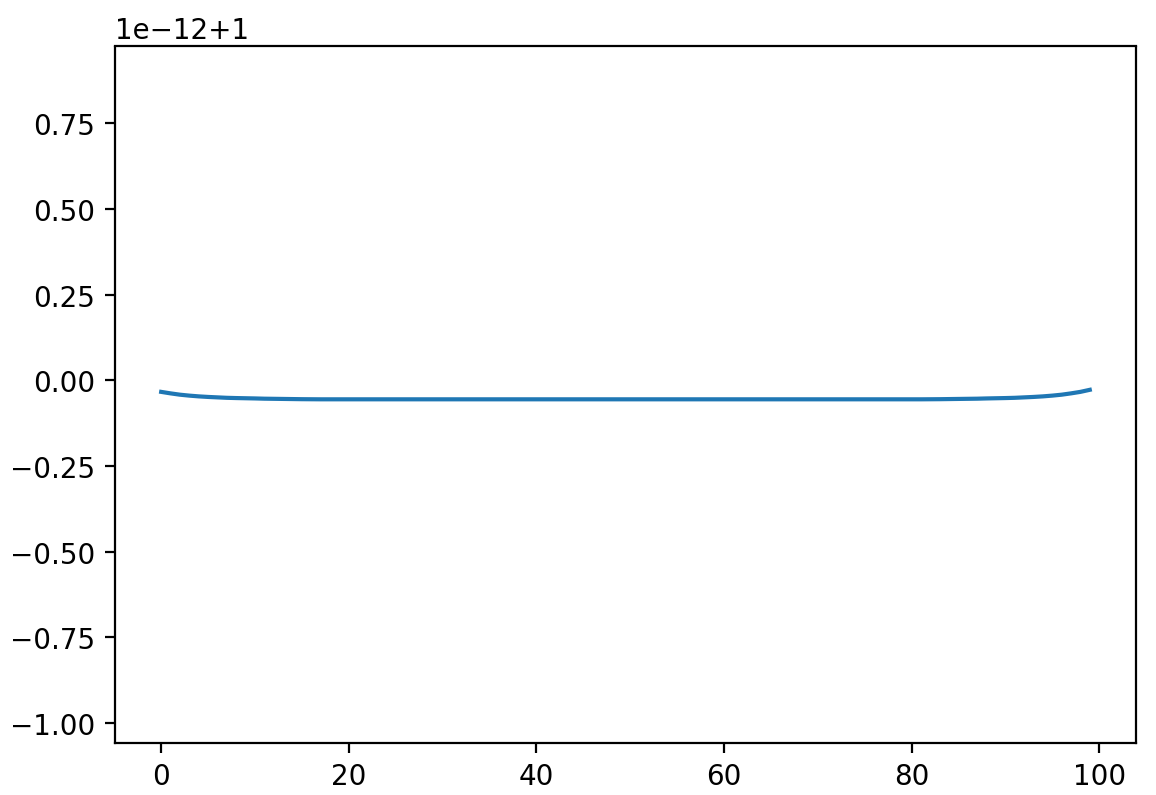
\includegraphics[width=\linewidth]{Fisher/f10000.png}
    \caption{$t=10000$}
  \end{subfigure}
\end{figure}

The Fisher equation (\ref{eq:fisher}) is related to the logistic equation (\ref{eq:logistic}) previously
described. The logistic equation can be thought of as the $R(\vec{q})$ given in the generalized
reaction diffusion equation (\ref{eq:genRD}) and the $\dfrac{\partial^2 u}{\partial t^2}$ is the 
$ - \underline{\underline{\mathbf{D}}} \nabla^2 \vec{q} $ of the general form. The fisher equation is not as
generalized as the logistic equation since the \say{carrying capacity} is 1; however, these equations are
still useful for illustrating the relation between reaction and reaction-diffusion systems.

\subsection{Cahn-Hilliard} \label{cahnhilliard}
\begin{singlespace}
  \begin{equation}\label{eq:cahnHilliard}
    \begin{split}
      \frac{\partial c}{\partial t} &= D \nabla^2 (c^3 -c -\gamma \nabla^2 c) \\
                                    &= D \nabla^2 \mu 
    \end{split}
  \end{equation}
  \begin{small}
$c$ is the concentration of the liquid \\
$D$ is the diffusion coefficient \\
$\sqrt{\gamma}$ is the length of the transition regions between the domain \\
$\mu = (c^3 - c -\gamma \nabla^2 c)$ is the called the chemical potential 
  \end{small}
\end{singlespace}

\begin{figure}[h]
  \caption{Cahn-Hilliard Examples at $t=2000$}
  \label{fig:cahnHilliardGraphs}
  \centering
  \begin{subfigure}[b]{.23\linewidth}
    
\includegraphics[width=\linewidth]{CahnHilliard/ch0.png}
    \caption{Initial Seed}
  \end{subfigure}
  \begin{subfigure}[b]{.23\linewidth}
    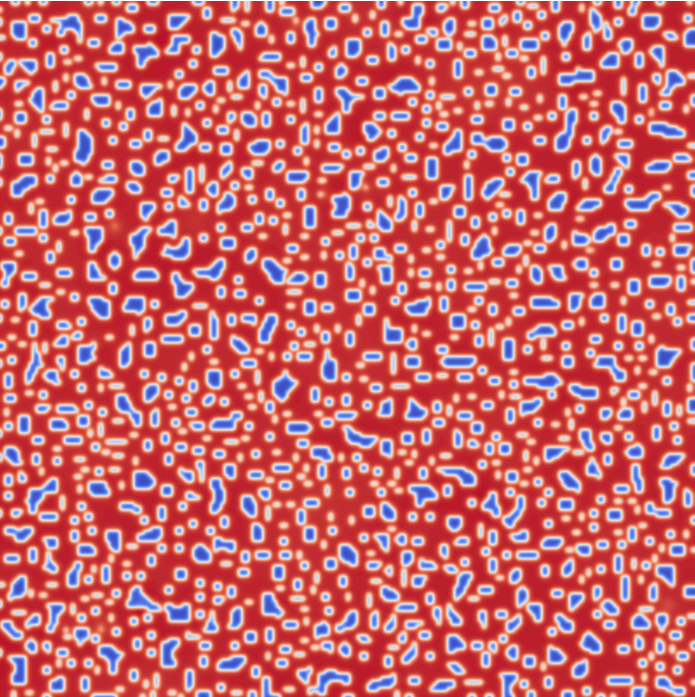
\includegraphics[width=\linewidth]{CahnHilliard/ch125.png}
    \caption{$\gamma=0.125$}
  \end{subfigure}
  \begin{subfigure}[b]{.23\linewidth}
    
\includegraphics[width=\linewidth]{CahnHilliard/ch375.png}
    \caption{$\gamma=0.375$}
  \end{subfigure}
  \begin{subfigure}[b]{.23\linewidth}
    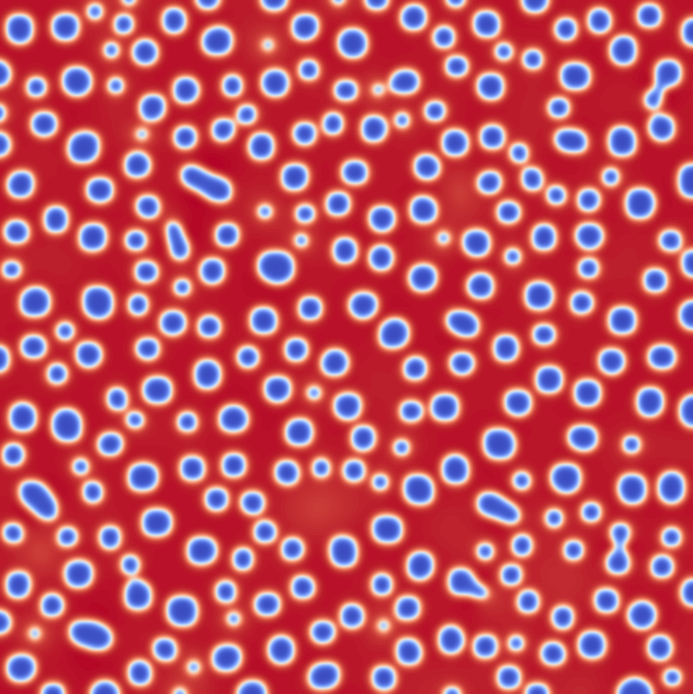
\includegraphics[width=\linewidth]{CahnHilliard/ch5.png}
    \caption{$\gamma=0.5$}
  \end{subfigure}
\end{figure}

The Cahn-Hilliard equation (\ref{eq:cahnHilliard}) is a 1 component, N dimensional system related to phase 
separation \citep{cahnhilliard}. Where fisher's equation (\ref{eq:fisher}) is about the phase transition in 1
dimension, which is a wave,
the Cahn-Hilliard equation can be used to describe the phase transition on a plane or any space,
$\mathbb{R}^n$. This system can be applied to a multitude of uses, a theme of reaction diffusion equations.
One such use is in high-strength alloys \citep{challoys}. An intuitive way of thinking about this process
despite losing some of the generality is thinking about the Cahn-Hilliard equation is as the interaction
between insoluble fluids. If the $\gamma$ in the chemical potential, $\mu$, is high enough as $t$ approaches
$\infty$ the two insoluble fluids completely separate. It is clear that the Cahn-Hilliard equation is very
useful for studying emulsions and solutions as shown by \cite{CHEmulsions} and other studies.  

\begin{singlespace}
  \begin{equation}\label{eq:grayscott}
    \begin{split}
      &\frac{\partial a}{\partial t} = d_a\nabla^2a − ab^2 + f(1−a) \\
      &\frac{\partial b}{\partial t} = d_b\nabla^2b + ab^2 − (k + f)b
    \end{split}
  \end{equation}
  \begin{equation}
    \begin{split}
      a + 3b &\rightarrow 3b \\
           b &\rightarrow p
    \end{split}
  \end{equation}
  \begin{small}
$d_a$ is the rate of growth for a \\
$d_b$ is the rate of growth for b \\
$f$ is the feed rate also keeps a from exceeding 1 \\
$k$ is the kill rate of b which is scaled by b to prevent it from being less than 0
  \end{small}
\end{singlespace}

\begin{figure}[h]
  \caption{Coral Simulation}
  \label{fig:coralProgression}
  \centering
  \begin{subfigure}[b]{.22\linewidth}
    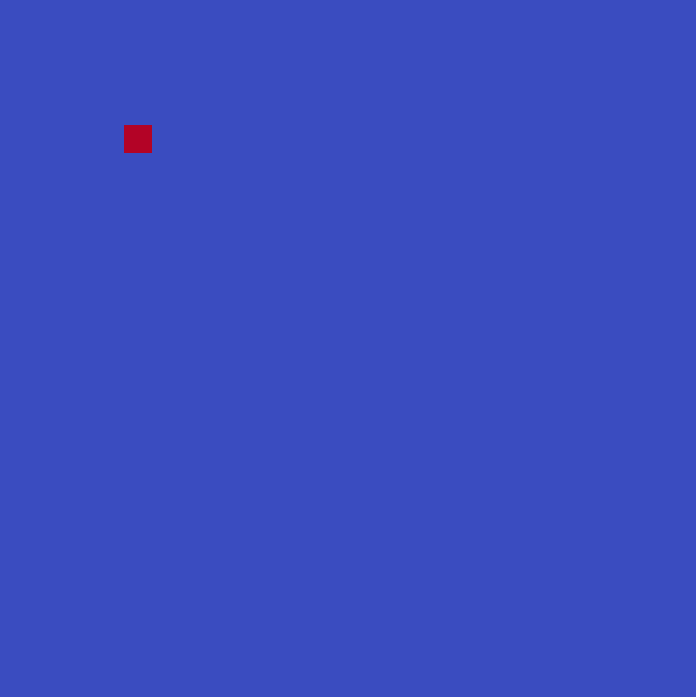
\includegraphics[width=\linewidth]{GrayScott/coral0.png}
    \caption{$r=0.1$}
  \end{subfigure}
  \begin{subfigure}[b]{.22\linewidth}
    
\includegraphics[width=\linewidth]{GrayScott/coral1000.png}
    \caption{$r=0.2$}
  \end{subfigure}
  \begin{subfigure}[b]{.22\linewidth}
    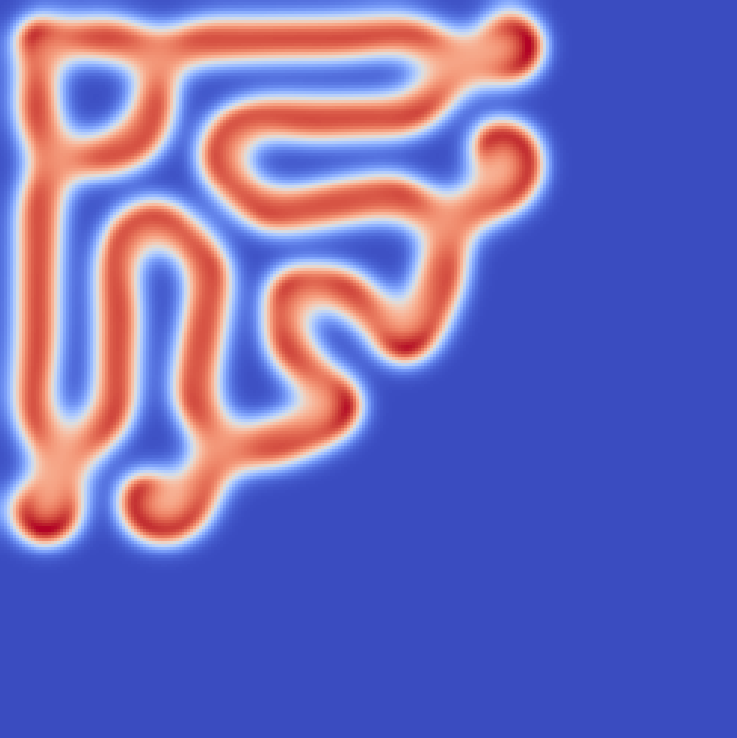
\includegraphics[width=\linewidth]{GrayScott/coral5000.png}
    \caption{$r=0.3$}
  \end{subfigure}
  \begin{subfigure}[b]{.22\linewidth}
    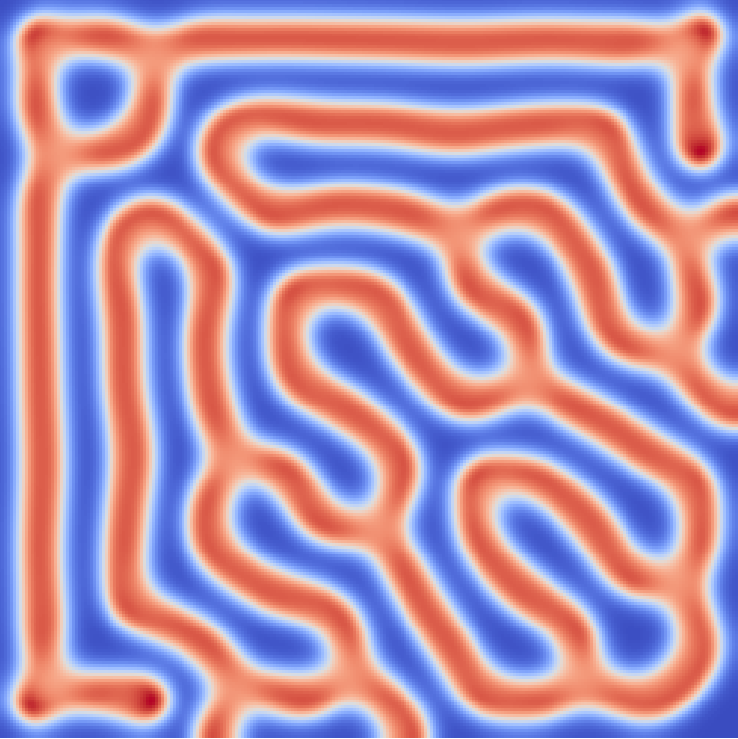
\includegraphics[width=\linewidth]{GrayScott/coral10000.png}
    \caption{$r=0.3$}
  \end{subfigure}
\end{figure}

The Gray-Scott Model the reaction diffusion equation for computational art. Originally it was for a modeling
a specific chemical reaction \citep{grayscott}; however, due to its generality and interesting patterns it
became used for making natural-looking patterns with a seed, example Gray-Scott lamp \citep{reactionLamp}. 
The original reaction takes in $a$ and $b$ then produces a, $p$, byproduct. $k$ is the rate that $b$ turns
into the nonreactive $p$ and $f$ is the rate that $a$ is added and the other components are removed.
It has also been picked up by computational artists. Its main uses are for modeling patterns in biology.
These
patterns, also known as Turing patterns, can be used to generate mitosis and spirals to zebrafish patterns. An example of the
differences between reaction and reaction diffusion systems is firstly the spatial component and secondly how
the patterns change given their environment. In animal Turing patterns, the area and type of skin effects the
pigment patterns. For leopards, the patterns for the patches are not homogeneous; around the center of their
sides the patches are normally larger and decrease in size as they go to the paws or face \citep{turingsCat}.

\section{Conclusion}


\bibliographystyle{apa}
\bibliography{EE}
\newpage
\section{Appendix}

\listoffigures

\lstinputlisting[language=Python, label={lst:surfaceCode}, caption={Surface}]{code/surface.py}
\lstinputlisting[language=Python, label={lst:gradientCode}, caption={Gradient}]{code/gradient.py}
\lstinputlisting[language=Python, label={lst:divergenceCode}, caption={Divergence}]{code/divergence.py}
\lstinputlisting[language=Python, label={lst:diffusionCode}, caption={Diffusion}]{code/diffusion.py}
\lstinputlisting[language=Python, label={lst:logisticCode, caption={Logistic Equation}}]{code/logistic.py}
\lstinputlisting[language=Python, label={lst:lotkaVolterraCode}, caption={Lotka-Volterra}]{code/lotkaVolterra.py}
\lstinputlisting[language=Python, label={lst:SIRCode}, caption={SIR}]{code/SIR.py}
\lstinputlisting[language=Python, label={lst:cahnHilliardCode}, caption={Cahn-Hilliard}]{code/cahnHilliard.py}
\lstinputlisting[language=Python, label={lst:grayScottCode}, caption={Gray-Scott}]{code/grayScott.py}
\end{document}
